\section{RB-Methoden für lineare koerzive Probleme}
\label{sec-3}

\subsection{Primales RB-Problem}

\begin{defn}[Reduzierte Basis, RB-Räume]
	Sei $S_N = \set{\mu_1,\cdots,\mu_N} \subset \p$ Menge von Parametern mit (o.B.d.A.) linear unabhängigen Lösungen $\set{u(\mu_i)}_{i=1}^N$ von $\prob[\mu_i]$.
	Dann ist $X_N := \spn{\set{u(\mu_i)}_{i=1}^N}$ ein sog.\ \emph{Lagrange-RB-Raum}.\\
	Sei $\mu^0 \in \p$ und $u(\mu)$ Lösung von $\prob[\mu^0]$ $k$-mal diffbar in Umgebung von $\mu^0$.
	Dann ist
	\[
		X_{k,\mu^0} := \spn{\set{\partial_\sigma u(\mu^0) : \sigma \in \N_0^p, |\sigma| \leq k}}
	\]
	ein \emph{Taylor-RB-Raum}.
	Eine Basis $\Phi_N = \set{\phi_1,\cdots,\phi_N} \subseteq X$ eines RB-Raums ist eine \emph{reduzierte Basis}.
\end{defn}

\begin{bem} \beginwithlistbem
	\begin{itemize}
		\item $\Phi_N$ kann direkt aus Snapshots $u(\mu^i)$ oder, für numerische Stabilität (siehe \ref{sec-3.7}), auch orthonormiert sein.
		\item Wahl der Parameter $\set{\mu^i}$ ist entscheidend für Güte des RB-Modells:\\
			Hier: zufällige oder äquidistante Menge ausreichend\\
			Später: intelligente Wahl durch a-priori Analysis oder Greedy-Verfahren
		\item Es ex. auch andere Arten von RB-Räumen (Hermite, POD).
			Gemeinsam ist diesen die Konstruktion aus Snapshots von $u$ bzw.\ $\partial_\sigma u$.
		\item Andere MOR-Techniken: $\Phi_N$ kann auch komplett unabhängig von Snapshots auf andere Weise konstruiert werden: Balanced Truncation, Krylov-Räume, etc.\ (siehe z.B.\ Antoulas: Approximation of large scale dynamical systems, SIAM 2004)
	\end{itemize}
\end{bem}

\begin{defn}[Reduziertes Problem $\rprob$]
	Sei eine Instanz von $\prob$ gegeben und $X_N \subseteq X$ ein RB-Raum.
	Zu $\mu \in \p$ ist die RB-Lösung $u_N(\mu) \in X_N$ und Ausgabe $s_N(\mu) \in \R$ gesucht mit
	\begin{align*}
		a(u_N(\mu),v;\mu) &= f(v;\mu) &\forall v \in X_N\\
		s_N(\mu) &= l(u_N;\mu)
	\end{align*}
\end{defn}

\begin{bem} \beginwithlistbem
	\begin{itemize}
		\item Wir nennen obiges ``primal'' weil im Fall $f \neq l$ oder $a$ asymmetrisch, kann mit Hilfe eines geeigneten dualen Problems bessere Schätzung für $s$ erreicht werden.
		\item Obiges ist ``Ritz-Galerkin''-Projektion im Gegensatz zu ``Petrov-Galerkin''-Projektion, welches für nicht-koerzive Probleme notwendig ist. $\leadsto$ \ref{sec-4}
	\end{itemize}
\end{bem}

\begin{satz}[Galerkin-Projektion, Galerkin-Orthogonalität] \label{3.3}
	Sei $P_\mu : X \to X_N$ die orthogonale Projektion bzgl.\ Energieskalarprodukt $\dotp\pdot\pdot_\mu$, \emph{sei $a$ symmetrisch} und $u(\mu)$, $u_N(\mu)$ Lösung von $\prob$ bzw.\ $\rprob$.
	Dann:
	\begin{enumerate}
		\item $u_N(\mu) = P_\mu u(\mu)$ ``Galerkin-Projektion''
		\item $\dotp{e(\mu)}{v}_\mu = 0$ $\forall v \in X_N$, wobei $e(\mu) := u(\mu) - u_N(\mu)$
	\end{enumerate}

	\begin{proof}
		Nach Aufgabe 1/Blatt 1 ist $P_\mu$ wohldefiniert, denn $(X,\dotp\pdot\pdot_\mu)$ ist Hilbertraum und $X_N \subseteq X$ abgeschlossen weil endlichdimensional.
		Orthogonale Projektion des Fehlers ergibt
		\begin{align*}
			& & \dotp{P_\mu u(\mu) - u(\mu)}{\phi_i}_\mu &= 0 & \forall i = 1,\cdots,N &\\
			& \Leftrightarrow & a(P_\mu u(\mu) - u(\mu), \phi_i; \mu) &= 0 & \forall i = 1,\cdots,N &\\
			& \Leftrightarrow & a(P_\mu u(\mu), \phi_i; \mu) &= a(u(\mu),\phi_i;\mu) = f(\phi_i;\mu) & \forall i = 1,\cdots,N &
		\end{align*}
		\begin{enumerate}
			\item also ist $P_\mu u(\mu)$ Lösung von $\rprob$
			\item $e(\mu)$ ist also Projektions-Fehler, orthogonal nach Aufgabe 1/Blatt 1
		\end{enumerate}
	\end{proof}
\end{satz}

\begin{bem}
	Für $a$ nichtsymmetrisch gilt immer noch folgende ``Galerkin-Orthogonalität''
	\[
		a(u-u_N,v;\mu) = 0 \quad \forall v \in X_N
	\]
	(auch wenn $a$ kein Skalarprodukt)
\end{bem}

\begin{satz}[Existenz und Eideutigkeit für $\rprob$]
	Zu $\mu \in \p$ ex. eindeutige Lösung $u_N(\mu) \in X_N$ und RB-Ausgabe $s_n(\mu) \in \R$ von $\rprob$.
	Diese sind beschränkt
	\begin{align*}
		\norm{u_N(\mu)} &\leq \frac{\norm{f(\pdot;\mu)}_{X'}}{\alpha(\mu)} \leq \frac{\bar\gamma_f}{\bar\alpha}\\
		\norm{s_N(\mu)} &\leq \norm{l(\pdot;\mu)} \norm{u_N(\mu)} \leq \frac{\bar\gamma_l \bar\gamma_f}{\bar\alpha}
	\end{align*}

	\begin{proof}
		Weil $X_N \subset X$ ist $a(\pdot,\pdot;\mu)$ stetig und koerziv auf $X_N$.
		\begin{align*}
			\alpha_N(\mu) &:= \inf_{v \in X_N} \frac{a(v,v;\mu)}{\norm{v}^2} \geq \inf_{v \in X} \frac{a(v,v;\mu)}{\norm{v}^2} = \alpha(\mu) > 0\\
			\gamma_N(\mu) &:= \sup_{u,v \in X_N} \frac{a(u,v;\mu)}{\norm u \norm v} \leq \sup_{u,v \in X} \frac{a(u,v;\mu)}{\norm u \norm v} = \gamma(\mu) < \infty
		\end{align*}
		analog $f$, $l$ stetig auf $X_N$. Existenz, Eindeutigkeit und Schranken folgen also mit Lax-Milgram analog zu 2.8.
	\end{proof}
\end{satz}

\begin{kor}[Lipschitz-Stetigkeit]
	Seien $f$, $l$ gleichmäßig beschränkt und $a$, $f$, $l$ Lipschitz-stetig bzgl.\ $\mu$, dann sind auch $u_N(\mu)$, $s_N(\mu)$ Lipschitz-stetig bzgl.\ $\mu$ mit $L_u$, $L_s$ wie in 2.15.

	\begin{proof}
		Analog zu 2.15 / Übung.
	\end{proof}
\end{kor}

\begin{satz}[Diskrete RB-Probleme] \label{3.6}
	Sei $\Phi_N = \set{\phi_1,\cdots,\phi_N}$ eine reduzierte Basis für $X_N$.
	Für $\mu \in \p$,
	\begin{align*}
		A_N(\mu) &:= \seq{a(\phi_j,\phi_i;\mu)}_{i,j=1}^N & \in \R^{N \times N}\\
		\ubar l_N(\mu) &:= \seq{l(\phi_i;\mu)}_{i=1}^N & \in \R^N\\
		\ubar f_N(\mu) &:= \seq{f(\phi_i;\mu)}_{i=1}^N & \in \R^N
	\end{align*}
	und $\ubar u_N = \seq{u_{N,i}}_{i=1}^N \in \R^N$ als Lösung von
	\begin{equation}
		A_N(\mu) \ubar u_N = \ubar f_N(\mu)
		\label{eq:3.1}
	\end{equation}
	Dann ist $u_N(\mu) := \sum_{i=1}^N u_{N,i} \, \phi_i$ und $s_N(\mu) := \ubar l_N^\top(\mu) \ubar u_N$.

	\begin{proof}
		Einsetzen und Linearität zeigt, dass
		\[
			a \left(\sum u_{N,j} \, \phi_j, \phi_i; \mu \right) = \seq{A_N(\mu) \ubar u_N}_i = \seq{\ubar f_N}_i = f(\phi_i;\mu)
		\]
	\end{proof}
\end{satz}

\begin{satz}[Kondition bei ONB und Symmetrie]
\label{3.7}
	Falls $a(\pdot,\pdot;\mu)$ symmetrisch und $\Phi_N$ ist ONB, so ist Kondition von \eqref{eq:3.1} unabhängig von $N$ beschränkt
	\[
		\op{cond}_2(A_N) := \norm{A_N}_2 \norm{A_N^{-1}}_2 \leq \frac{\gamma(\mu)}{\alpha(\mu)}
	\]

	\begin{proof}
		Wegen Symmetrie gilt
		\begin{equation}
			\op{cond}_2(A_N) = \frac{|\lambda_\text{max}|}{|\lambda_\text{min}|}
			\label{eq:3.2}
		\end{equation}
		mit betragsmäßig größtem/kleinstem Eigenwert $\lambda_\text{max}$/$\lambda_\text{min}$ von $A_N(\mu)$.
		Sei $\ubar u_\text{max} = \seq{u_i}_{i=1}^N \in \R^N$ Eigenvektor zu $\lambda_\text{max}$ und
		\[
			u_\text{max} := \sum_{i=1}^N u_i \, \phi_i \quad \in X_N
		\]
		Dann gilt
		\begin{align*}
			\lambda_\text{max} \norm{\ubar u_\text{max}}^2 &= \lambda_\text{max} \ubar u_\text{max}^\top \ubar u_\text{max} = \ubar u_\text{max}^\top A_N \ubar u_\text{max}\\
			&= \sum_{i,j=1}^N u_i u_j \, a(\phi_j,\phi_i;\mu) = a\left(\sum_j u_j \phi_j, \sum_i u_i \phi_i; \mu\right)\\
			&= a(u_\text{max},u_\text{max};\mu) \leq \gamma(\mu) \norm{u_\text{max}}^2
		\end{align*}
		Wegen
		\[
			\norm{u_\text{max}}^2 = \dotp{\sum u_i \phi_i}{\sum u_j \phi_j} = \sum u_i u_j \dotp{\phi_i}{\phi_j} = \sum u_i^2 = \norm{\ubar u_\text{max}}^2
		\]
		folgt $|\lambda_\text{max}| \leq \gamma(\mu)$. Analog zeigt man $|\lambda_\text{min}| \geq \alpha(\mu)$ also folgt mit \eqref{eq:3.2} die Behauptung.
	\end{proof}
\end{satz}

\begin{bem}[Unterschied FEM zu RB]
	Es bezeichne $A_h(\mu) \in \R^{H \times H}$ die FEM Matrix (oder FV/FD).
	\begin{enumerate}
		\item Die RB-Matrix $A_N(\mu) \in \R^{H \times H}$ ist klein aber typischerweise vollbesetzt im Gegensatz zur großen aber dünnbesetzten Matrix $A_h$.
		\item Die Kondition von $A_N$ verschlechtert sich nicht mit wachsendem N (falls eine ONB verwendet wird), während die Konditionszahl von $A_h$ typischerweise polynomiell in $H$ wächst, also schlechter wird.
	\end{enumerate}
\end{bem}

\begin{satz}[Reproduktion von Lösungen] \label{3.8}
	Seien $u(\mu)$, $u_N(\mu)$ Lösungen von $\prob$ bzw.\ $\rprob$, $\ubar e_i \in \R^n$ $i$-ter Einheitsvektor
	\begin{enumerate}
		\item Falls $u(\mu) \in X_N \quad \Rightarrow \quad u_N(\mu) = u(\mu)$
		\item Falls $u(\mu) = \phi_i \in \Phi_N \quad \Rightarrow \quad \ubar u_N(\mu) = \ubar e_i \in \R^N$
	\end{enumerate}

	\begin{proof} \beginwithlistbew
		\begin{enumerate}
			\item Mit $u(\mu)$, $u_N(\mu) \in X_N \Rightarrow e := u(\mu) - u_N(\mu) \in X_N$.
				Wegen Galerkin-Orthogonalität ($a(e,v;\mu) = 0 \; \forall v \in X_N)$ und Koerzivität folgt:
				\[
					0 = a(e,e;\mu) \geq \underbrace{\alpha(\mu)}_{> 0} \underbrace{\norm{e}^2}_{\geq 0} \quad \Rightarrow \quad \norm{e} = 0 \Rightarrow e = 0 \Rightarrow u = u_N
				\]
			\item $u_N(\mu) = \phi_i$, nach i).
				Mit Eindeutigkeit der Basisexpansion folgt die Behauptung.
		\end{enumerate}
	\end{proof}
\end{satz}

\begin{bem} \beginwithlistbem
	\begin{itemize}
		\item Reproduktion von Lösungen ist grundlegende Konsistenzeigenschaft.
			Es gilt trivialerweise falls/sobald Fehlerschranken vorliegen, aber für komplexe RB-Probleme ohne Fehlerschranken ist obiges ein guter Test.
		\item Validierung für Programmcode: Wähle Basis aus Snapshots $\phi_i = u(\mu^i)$, $i=1,\dots,N$, ohne Orthonormierung, dann muss $\ubar u_N(\mu^i) = \ubar e_i \in \R^N$ ein Einheitsvektor sein.
	\end{itemize}
\end{bem}

\subsection{Fehleranalyse}

\begin{satz}[Céa, Beziehung zur Bestapproximation] \label{3.9}
	Für alle $\mu \in \p$ gilt
	\[
		\norm{u(\mu)-u_N(\mu)} \leq \frac{\gamma(\mu)}{\alpha(\mu)} \inf_{v \in X} \norm{u-v}
	\]

	\begin{proof}
		$\forall v \in X_N$ mit Stetigkeit und Koerzivität
		\begin{align*}
			\alpha \norm{u-u_N}^2 &\leq a(u-u_N,u-u_N) = a(u-u_N,u-v) + \underbrace{a(u-u_N,v-u_N)}_{= 0 \text{ (Galerkin-Orth.)}}\\
			&\leq \gamma(\mu) \norm{u-u_N} \norm{u-v}
		\end{align*}
		Division durch $\alpha$, $\norm{u-u_N}$ liefert
		\[
			\norm{u-u_N} \leq \frac{\gamma}{\alpha} \norm{u-v}
		\]
		also Behauptung durch Infimum-Bildung.
	\end{proof}
\end{satz}

\begin{bem} \beginwithlistbem
	\begin{enumerate}
		\item Ähnliche Bestapproximationsaussagen gelten auch für andere Interpolationstechniken, aber die zugehörige Lebesgue-Konstante divergiert meist mit wachsender Dimension $N$.
			Obiges ist konzeptioneller Vorteil von Galerkin-Projektion über anderen Interpolationstechniken, da $\frac{\gamma}{\alpha}$ unabhängig von $N$ beschränkt bleibt.
			``Quasi-Optimalität'' der Galerkin-Projektion/des RB-Ansatzes.
		\item Falls $a(\pdot,\pdot;\mu)$ zusätzlich symmetrisch ist, kann um eine ``Wurzel'' verbessert werden mittels Normäquivalenz \ref{2.5} und Bestapproximation der orthogonalen Projektion (Aufg. 1/Blatt 1)
			\begin{align*}
				\sqrt{\alpha} \norm{u-u_N} &\stackrel{\ref{2.5}}{\leq} \norm{u-u_N}_\mu = \norm{u-P_\mu u}_\mu = \inf_{v \in X_N} \norm{u-v}_\mu \stackrel{\ref{2.5}}{\leq} \sqrt{\gamma} \inf_{v \in X_N} \norm{u-v}\\
				\Rightarrow \; \norm{u-u_N} &\leq \sqrt{\frac \gamma \alpha} \inf_{v \in X_N} \norm{u-v}
			\end{align*}
		\item Implikation von \ref{3.9}: Wähle guten Approximationsraum $X_N$, so wird Galerkin-Projektion/RB-Approximation auch garantiert gut sein.
	\end{enumerate}
\end{bem}

\begin{satz}[Ausgabe und Bestapproximation] \label{3.10} \beginwithlist
	\begin{enumerate}
		\item Für alle $\mu \in \p$ gilt
			\[
				|s(\mu)-s_N(\mu)| \leq \norm{l(\pdot;\mu)}_{X'} \frac{\gamma(\mu)}{\alpha(\mu)} \inf_{v \in X_N} \norm{u-v}
			\]
		\item Für den sog.\ ``compliant'' Fall (d.h.\ $a(\pdot,\pdot;\mu)$ symmetrisch und $l = f$) gilt sogar
			\begin{align*}
				0 \leq s(\mu)-s_N(\mu) &= \norm{u-u_N}_\mu^2\\
				&= \inf_{v \in X_N} \norm{u-v}_\mu^2\\
				&\leq \gamma(\mu) \inf_{v \in X_N} \norm{u-v}^2
			\end{align*}
	\end{enumerate}

	\begin{proof} \beginwithlistbew
		\begin{enumerate}
			\item Klar mit Céa, Bestapproximation und Linearität
				\[
					|s(\mu)-s_N(\mu)| = |l(u)-l(u_N)| = |l(u-u_N)| \leq \norm l \norm{u-u_N} \leq \norm{l} \frac{\gamma}{\alpha} \inf_{v \in X_N} \norm{u-v}
				\]
			\item Wegen $a(\pdot,\pdot;\mu)$ symmetrisch gilt wie in voriger Bemerkung
				\begin{equation} \label{eq:3.3}
					\norm{u-u_N}_\mu = \norm{u-P_\mu u}_\mu = \inf_{v \in X_N} \norm{u-v}
				\end{equation}
				Damit
				\begin{align*}
					s(\mu) - s_N(\mu) &= l(u)-l(u_N) \stackrel{f=l}{=} f(u) - f(u_N) = f(u-u_N)\\
					&= a(u,u-u_N) - \underbrace{a(u_N,u-u_N)}_{=0 \text{ (Gal.-Orth./Symm.)}} = \norm{u-u_N}_\mu^2\\
					&\stackrel{\ref{3.3}}{=} \inf_{v \in X_N} \norm{u-v}_\mu^2\\
					&\stackrel{\ref{2.5}}{\leq} \gamma \inf_{v \in X_N} \norm{u-v}^2
				\end{align*}
				Also insbesondere $s-s_N = \norm{u-u_N}_\mu^2 \geq 0$.
		\end{enumerate}
	\end{proof}
\end{satz}

\begin{bem} \beginwithlistbem
	\begin{itemize}
		\item Im ``compliant'' Fall ist der Ausgabefehler i.A.\ sehr klein, da das Quadrat des RB-Fehlers eingeht.
		\item Im ``nicht-compliant'' Fall geht der RB-Fehler nur linear in die Schranke ein, das wird später durch primal-duale Technik verbessert.
		\item Aus ii) folgt nicht nur Fehlerschranke, sondern sogar Vorzeichen-Information, $s_N(\mu)$ ist untere Schranke für $s$.
	\end{itemize}
\end{bem}

\begin{kor}[Monotoner Fehlerabfall in Energienorm] \label{3.11}
	Falls $a(\pdot,\pdot;\mu)$ symmetrisch, $\seq{X_N}_{N=1}^{N_\text{max}}$ Folge von RB-Räumen, mit $X_N \subseteq X_{N'}$, $\forall N \leq N'$ (``hierarchische Räume'') und für $\mu \in \p$ setze $e_{u,N} := u(\mu)-u_N(\mu)$, $e_{s,N} := s(\mu)-s_N(\mu)$.
	\begin{enumerate}
		\item Dann ist $\seq{\norm{e_{u,N}}_\mu}_{N=1}^{N_\text{max}}$ monoton fallend.
		\item Falls $l=f$ (also ``compliant'' Fall) ist $e_{s,N}$ monoton fallend.
	\end{enumerate}

	\begin{proof} \beginwithlistbew
		\begin{enumerate}
			\item Mit \eqref{eq:3.3} gilt für $N \leq N'$
				\[
					\norm{e_{u,N}}_\mu = \norm{u-u_N}_\mu \stackrel{\eqref{eq:3.3}}{=} \inf_{v \in X_N} \norm{u-v}_\mu \geq \inf_{v \in X_{N'}} \norm{u-v}_\mu \stackrel{\eqref{eq:3.3}}{=} \norm{e_{u,N'}}_\mu
				\]
			\item Mit Satz \ref{3.10} ii) gilt
				\[
					e_{s,N} = \norm{e_{u,N}}_\mu^2 \text{, also Behauptung folgt mit i)}
				\]
		\end{enumerate}
	\end{proof}
\end{kor}

\begin{bem} \beginwithlistbem
	\begin{itemize}
		\item ``Worst-case'' ist Stagnation des Fehlers (unrealistisch, jeder neue Basisvektor müsste orthogonal zum Fehler $e_N(\mu)$ sein).
			In Praxis ist bei geschickter Basiswahl und ``glatten'' Problemen exponentielle Konvergenz zu erwarten, siehe Basisgenerierung, §\ref{sec-3.4}.
		\item Monotonie gilt nicht notwendigerweise bezüglich anderen Normen trotz Normäquivalenz
			\[
				c \norm{e_{u,N}}_\mu \leq \norm{e_{u,N}} \leq C \norm{e_{u,N}}_\mu \text{, mit $c$, $C$ unabhängig von $N$}
			\]
			Fehlernorm $\norm{e_{u,N}}$ kann gelegentlich anwachsen, bleibt aber in einem ``Korridor'', welcher monoton fällt.
	\end{itemize}

	\begin{figure}[H]
		\centering\small
		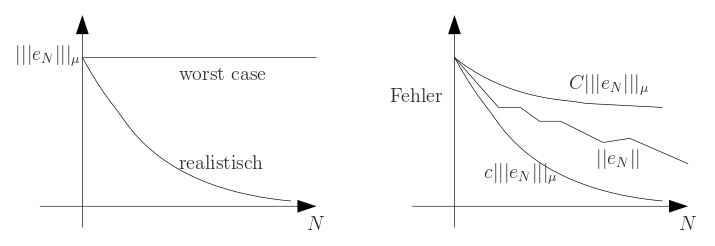
\includegraphics[width = 0.75 \textwidth]{Bilder/FehlerabfallEnergienorm.png}
		\caption{Fehlerabfall mit wachsender reduzierter Dimension.}{(aus B. Haasdonk, Reduzierte-Basis-Methoden, Skript zur Vorlesung SS 2011, Universität Stuttgart, IANS-Report 4/11, 2011.)}
		\label{fig:FehlerabfallEnergienorm}
	\end{figure}
\end{bem}

\begin{bem}[Gleichmäßige Konvergenz von Lagrange RB-Ansatz] \beginwithlistbem
	\begin{itemize}
		\item Sei $\p$ kompakt und $S_N := \set{\mu^1,\dots,\mu^N} \subset \p$, $N \in \N$, sodass die sog.\ Füll-Distanz (fill-distance) $h_N$ gegen 0 geht:
			\begin{align*}
				h_N &:= \sup_{\mu \in \p} \dist(\mu, S_N), \quad \dist(\mu,S_N) := \min_{\mu' \in S_N} \norm{\mu - \mu'}\\
				\lim_{N \to \infty} h_N &= 0
			\end{align*}
		\item Falls $u(\mu)$, $u_N(\mu)$ Lipschitz-stetig mit Lipschitz-Konstante $L_u$ unabhängig von $N$, so folgt für alle $N$, $\mu$ und ``nächstes'' $\mu^* := \arg\min_{\mu' \in S_N} \norm{\mu-\mu'}$:
			\begin{align*}
				\norm{u(\mu)-u_N(\mu)} &\leq \norm{u(\mu)-u(\mu^*)} + \norm{u(\mu^*)-u_N(\mu^*)} + \norm{u_N(\mu^*)-u_N(\mu)}\\
				&\leq L_u \underbrace{\norm{\mu-\mu^*}}_{\leq h_N} + 0 + L_u \underbrace{\norm{\mu - \mu^*}}_{\leq h_N} \leq 2 L_u h_N
			\end{align*}
		\item Also folgt uniforme Konvergenz
			\[
				\lim_{N \to \infty} \sup_{\mu \in \p} \norm{u(\mu)-u_N(\mu)} = 0
			\]
			\item Jedoch Konvergenzrate linear in $h_N$ ist nicht praktisch bedeutsam, weil $h_N$ sehr langsam mit $N$ abfällt, also muss $N$ sehr groß sein, um kleinen Fehler zu garantieren.
			\item Wir werden sehen, dass bei gleichmäßig koerziven Problemen und geschickter Wahl der $\mu^i$ sogar exponentielle Konvergenz erreicht wird.
	\end{itemize}
\end{bem}

\begin{lemma}[Fehler-Residuums-Beziehung] \label{3.12}
	Für $\mu \in \p$ definieren wir mittels der RB-Lösung $u_N$ das Residuum $r(\pdot;\mu) \in X'$ bzw.\ seinen Riesz-Repräsentanten $v_r(\mu) \in X$
	\[
		\dotp{v_r(\mu)}{v}_X := r(v;\mu) := f(v;\mu) - a(u_N(\mu),v;\mu) \quad \forall v \in X
	\]
	Dann erfüllt der Fehler $e(\mu) := u(\mu)-u_N(\mu)$
	\[
		a(e(\mu),v;\mu) = r(v;\mu) \quad \forall v \in X
	\]

	\begin{proof}
		$a(e(\mu),v;\mu) = \underbrace{a(u,v)}_{f(v)} - a(u_N,v) = r(v)$
	\end{proof}
\end{lemma}

\begin{bem} \beginwithlistbem
	\begin{itemize}
		\item Fehler erfüllt ``$\prob$ mit Residuum als rechte Seite''
		\item Insbesondere ist $r(v;\mu) = 0$ $\forall v \in X_N$ (wegen Galerkin-Orthogonalität)
		\item $r(\pdot;\mu) = 0 \quad \Rightarrow \quad e = 0$
	\end{itemize}
\end{bem}

\begin{satz}[A-posteriori Fehlerschätzer, absoluter Fehler] \label{3.13}
	Sei $\mu \in \p$, $u(\mu)$ bzw.\ $u_N(\mu)$ Lösung von $\prob$, $\rprob$ und $e=u-u_N$.
	Sei $\alpha_{LB}(\mu)$ eine untere Schranke für $\alpha(\mu)$ und $v_r \in X$ Riesz-Repräsentant von $r(\pdot;\mu)$ aus Lemma \ref{3.12}.
	Dann gelten folgende Schranken
	\begin{enumerate}
		\item Fehler in Energienorm
			\[
				\norm{e(\mu)}_\mu \leq \Delta_N^{en}(\mu) := \frac{\norm{v_r}}{\sqrt{\alpha_{LB}(\mu)}}
			\]
		\item Fehler in $X$-Norm $\norm\pdot$
			\[
				\norm{e(\mu)} \leq \Delta_N(\mu) := \frac{\norm{v_r}}{\alpha_{LB}(\mu)}
			\]
		\item Ausgabefehler
			\[
				|s(\mu)-s_N(\mu)| \leq \Delta_{N,s}(\mu) := \norm{l(\pdot;\mu)} \Delta_N(\mu)
			\]
	\end{enumerate}

	\begin{proof} \beginwithlistbew
		\begin{enumerate}
			\item Normäquivalenz \ref{2.5} impliziert
				\[
					\norm e \leq \frac{\norm{e}_\mu}{\sqrt{\alpha_{LB}(\mu)}}
				\]
				Damit folgt
				\[
					\norm{e}_\mu^2 = a_s(e,e) = a(e,e) = r(v) = \dotp{v_r}{e} \leq \norm{v_r} \norm{e} \leq \frac{\norm{v_r}}{\sqrt{\alpha_{LB}(\mu)}}
				\]
				Division durch $\norm{e}_\mu$ liefert die Behauptung i).
			\item Koerzivität liefert
				\[
					\alpha_{LB}(\mu) \norm{e}^2 \leq a(e,e) = r(e) = \dotp{v_r}{e} \leq \norm{v_r} \norm{e}
				\]
				Division durch $\alpha_{LB}$ und $\norm e$ liefert ii).
			\item Stetigkeit von $l$ liefert
				\[
					|s(\mu)-s_N(\mu)| = |l(u-u_N;\mu)| \leq \norm{l} \norm{u-u_N} \stackrel{ii)}{\leq} \norm{l} \Delta_N
				\]
		\end{enumerate}
	\end{proof}
\end{satz}

\begin{bem} \beginwithlistbem
	\begin{itemize}
		\item $\alpha_{LB}(\mu)$ soll eine \emph{schnell berechenbare} untere Schranke an $\alpha(\mu)$ sein, z.B.\ $\alpha_{LB}(\mu) := \bar \alpha$ falls $\bar \alpha$ bekannt, andere Möglichkeiten folgen später (``min $\Theta$'', ``SCM'').
		\item $\Delta_N$ ist also immer um Faktor $\sqrt{\alpha_{LB}(\mu)}$ schlechter.
		\item Beschränkung des Fehlers durch Residuums-Norm ist bekannte Technik aus FEM, um FEM-Lösung $u_h$ gegen Sobolev-Raum Lösung $u$ abzuschätzen.
			In diesem Fall ist $X$ $\infty$-dimensional und Residuums-Norm algorithmisch nicht berechenbar.
			In RB-Methoden wird $\norm{v_r}$ eine \emph{berechenbare} Größe sobald $X$ endlich-dimensional, z.B.\ FEM-Raum, ist.
			Für Residuum ist $u_N(\mu)$ erforderlich, daher sind Schranken ``\emph{a posteriori}''.
		\item Allgemeines Vorgehen (und alternative Begründung für ii)) zur Herleitung von Fehlerschranken: Zeige, dass Fehler $e$ erfüllt $\prob$ mit rechter Seite, genannt $r$ (Residuum), wende a-priori Stabilitätsaussage an:
			\[
				\norm{e} \leq \frac{\norm r}{\alpha(\mu)} \quad \text{z.B.\ Lax-Milgram}
			\]
			und erhalte berechenbare Größe durch Wahl $X=X_{FEM}$ und untere Schranke $\alpha_{LB}(\mu) \leq \alpha(\mu)$.
		\item Weil die Schranken beweisbare obere Schranken an Fehler darstellen, nennt man sie ``rigorose'' Fehlerschranken (vgl.\ ``zuverlässige'' Schätzer in FEM, bei denen jedoch die Konstante unbekannt ist).
		\item Fehlerschranken liefern eine Absicherung für RB-Methoden, ``certified'' RB-Methode, im Gegensatz zu vielen anderen Reduktionsmethoden (z.B.\ Krylov-Raum-Methoden).
		\item Ausgabefehler ist grob, indem $\Delta_N$ nur linear eingeht.
			Verbesserungen können für den ``compliant'' Fall oder mit primal-dual Techniken erreicht werden. ($\leadsto$ §\ref{sec-3.5})
	\end{itemize}
\end{bem}

\begin{kor}[Verschwindende Fehlerschranke] \label{3.14}
	Falls $u(\mu) = u_N(\mu)$ dann ist $\Delta_N(\mu) = \Delta_N^{en}(\mu) = \Delta_{N,s}(\mu) = 0$

	\begin{proof}
		\[
			0 = a(0,v;\mu) = a(e,v;\mu) = r(v;\mu)
		\]
		\[
			\Rightarrow r \equiv 0 \Rightarrow \norm{v_r} = 0 \Rightarrow \Delta_N = \Delta_N^{en} = \Delta_{N,s} = 0
		\]
	\end{proof}
\end{kor}

\begin{bem} \beginwithlistbem
	\begin{itemize}
		\item Dies ist initialer Wunsch an eine Fehlerschranke: diese soll verschwinden falls exakte Approximation vorliegt.
			Dies ist Grundlage dafür, dass der Faktor der Überschätzung endlich ist.
		\item Aussage ist trivial für \emph{effektive} Fehlerschätzer (sehen wir bald), aber in komplexen Problemen kann \ref{3.14} schon das maximal erreichbare sein.
		\item \ref{3.14} ist wieder sinnvoll um Programmcode zu validieren.
	\end{itemize}
\end{bem}

\begin{satz}[A-posteriori Fehlerschranken, relative Fehler] \label{3.15}
	Mit Bezeichnungen/Voraussetzungen aus \ref{3.13} und unter Annahme, dass alle Brüche im Folgenden wohldefiniert sind, gilt:
	\begin{enumerate}
		\item Für den relativen Fehler gilt in Energienorm:
			\[
				\frac{\norm{e(\mu)}_\mu}{\norm{u(\mu)}_\mu} \leq \Delta_N^{en,rel}(\mu) := 2 \frac{\norm{v_r}}{\sqrt{\alpha_{LB}(\mu)}} \cdot \frac{1}{\norm{u_N(\mu)}_\mu} \quad \text{falls} \quad \Delta_N^{en,rel} \leq 1
			\]
		\item Für den relativen Fehler gilt in $X$-Norm:
			\[
				\frac{\norm{e(\mu)}}{\norm{u(\mu)}} \leq \Delta_N^{rel}(\mu) := 2 \frac{\norm{v_r}}{\alpha_{LB}(\mu)} \cdot \frac{1}{\norm{u_N(\mu)}} \quad \text{falls} \quad \Delta_N^{rel} \leq 1
			\]
	\end{enumerate}

	\begin{proof} \beginwithlistbew
		\begin{enumerate}
			\item Falls $\Delta_N^{en,rel}(\mu) \leq 1$, so ist
				\begin{align*}
					\left| \frac{\norm{u}_\mu-\norm{u_N}_\mu}{\norm{u_N}_\mu} \right| &\stackrel{\Delta \text{-Ungl.}}{\leq} \frac{\norm{u-u_N}_\mu}{\norm{u_N}_\mu} = \frac{\norm{e}_\mu}{\norm{u_N}_\mu} \stackrel{\ref{3.13} \text{ i)}}{\leq} \frac{\norm{v_r}}{\sqrt{\alpha_{LB}(\mu)} \norm{u_N}_\mu}\\
					&= \frac 1 2 \Delta_N^{en,rel}(\mu) \leq \frac 1 2
				\end{align*}
				Falls $\norm{u_N}_\mu > \norm{u}_\mu$ gilt $\norm{u_N}_\mu-\norm{u}_\mu \leq \frac 1 2 \norm{u_N}_\mu$ also
				\[
					\frac 1 2 \norm{u_N}_\mu \leq \norm{u}_\mu \tag{$*$}
				\]
				Falls $\norm{u}_\mu \geq \norm{u_N}_\mu$, so ist ($*$) klar.
				Damit folgt
				\[
					\frac{\norm{e}_\mu}{\norm{u}_\mu} \stackrel{\ref{3.13} \text{ i)}}{\leq} \frac{\norm{v_r}}{\sqrt{\alpha_{LB}}} \cdot \frac{1}{\norm{u}_\mu} \stackrel{(*)}{\leq} \frac{\norm{v_r}}{\sqrt{\alpha_{LB}}} \cdot \frac{1}{\norm{u_N}_\mu} \cdot 2 = \Delta_N^{en,rel}(\mu)
				\]
			\item analog zu i).
		\end{enumerate}
	\end{proof}
\end{satz}

\begin{bem} \beginwithlistbem
	\begin{itemize}
		\item Analog folgt auch relativer Ausgabefehlerschätzer
			\[
				\frac{|s(\mu)-s_N(\mu)|}{|s(\mu)|} \leq \Delta_{N,s}^{rel}(\mu) := \frac{\norm{l(\pdot;\mu)} \cdot \Delta_N}{|s_N(\mu)|} \cdot 2 \quad \text{falls} \quad \Delta_{N,s}^{rel}(\mu) \leq 1
			\]
		\item Relative Fehlerschranken sind nur mit Zusatzbedingung ($\Delta_*^{rel} \leq 1$) gültig.
			Diese Bedingung ist jedoch konkret überprüfbar.
			Falls $\Delta_N^{rel}(\mu) > 1$, sollte der RB-Raum verbessert werden.
	\end{itemize}
\end{bem}

\begin{satz}[Effektivität der Fehlerschranken] \label{3.16}
	Mit Bezeichnungen aus \ref{3.13} sei $u(\mu) \neq u_N(\mu)$ und $\gamma_{UB}(\mu) < \infty$ eine obere Schranke an $\gamma(\mu)$.
	Dann sind die \emph{Effektivitäten} $\eta_N^{en}(\mu)$ und $\eta_N(\mu)$ definiert und beschränkt durch
	\begin{enumerate}
		\item
			\[
				\eta_N^{en}(\mu) := \frac{\Delta_N^{en}(\mu)}{\norm{e}_\mu} \leq \frac{\gamma_{UB}(\mu)}{\alpha_{LB}(\mu)}
			\]
			Falls $a(\pdot,\pdot;\mu)$ symmetrisch, gilt sogar $\eta_N^{en}(\mu) \leq \sqrt{\frac{\gamma_{UB}(\mu)}{\alpha_{LB}(\mu)}}$
		\item
			\[
				\eta_N(\mu) := \frac{\Delta_N(\mu)}{\norm{e}_\mu} \leq \frac{\gamma_{UB}(\mu)}{\alpha_{LB}(\mu)}
			\]
	\end{enumerate}

	\begin{proof} \beginwithlistbew
		\begin{enumerate}
			\setcounter{enumi}{1}
			\item $\norm{v_r}^2 = \dotp{v_r}{v_r} = r(v_r) = a(e,v_r) \leq \gamma_{UB}(\mu) \norm{e} \norm{v_r}$
				\begin{equation} \label{eq:3.4}
					\norm{v_r} \leq \gamma_{UB}(\mu) \norm{e}
				\end{equation}
				Damit
				\[
					\frac{\Delta_N(\mu)}{\norm{e}} = \frac{\norm{v_r}}{\alpha_{LB}} \cdot \frac{1}{\norm{e}} \stackrel{\eqref{eq:3.4}}{\leq} \frac{\gamma_{UB}}{\alpha_{LB}} \cdot \frac{\norm e}{\norm e}
				\]
			\setcounter{enumi}{0}
			\item
				\[
					\frac{\Delta_N^{en}(\mu)}{\norm{e}_\mu} = \frac{\norm{v_r}}{\sqrt{\alpha_{LB}}} \cdot \frac{1}{\underbrace{\norm{e}_\mu}_{\geq \sqrt{\alpha_{LB}} \cdot \norm{e}}} \leq \frac{\norm{v_r}}{\alpha_{LB}} \cdot \frac{1}{\norm{e}} \stackrel{\text{ii)}}{\leq} \frac{\gamma_{UB}}{\alpha_{LB}}
				\]
				Falls $a(\pdot,\pdot)$ symmetrisch, gilt wegen Normäquivalenz
				\[
					\norm{v_r}_\mu \leq \sqrt{\gamma_{UB}} \norm{v_r}
				\]
				und
				\[
					\norm{v_r}^2 = a(e,v_r) \stackrel{\text{CS}}{\leq} \norm{e}_\mu \norm{v_r}_\mu \quad \Rightarrow \quad \norm{v_r} \leq \norm{e}_\mu \cdot \sqrt{\gamma_{UB}}
				\]
				Damit
				\[
					\frac{\Delta_N^{en}(\mu)}{\norm{e}_\mu} = \frac{\norm{v_r}}{\sqrt{\alpha_{LB}}} \cdot \frac{1}{\norm{e}_\mu} \leq \frac{\norm{e}_\mu \cdot \sqrt{\gamma_{UB}}}{\sqrt{\alpha_{LB}} \cdot \norm{e}_\mu}
				\]
		\end{enumerate}
	\end{proof}
\end{satz}

\begin{bem} \beginwithlistbem
	\begin{itemize}
		\item Wir nennen $\Delta_N$, $\Delta_N^{en}$ daher ``effektive'' Fehlerschranken weil Faktor der Überschätzung höchstens $\frac{\gamma_{UB}}{\alpha_{LB}}$ beträgt.
		\item ``Rigorosität'' also äquivalent mit $\eta_N(\mu) \geq 1$.
		\item Für den Ausgabefehler $\Delta_{N,s}(\mu)$ ohne weitere Annahmen keine Effektivität beweisbar.
			Tatsächlich kann $\frac{\Delta_{N,s}}{|s-s_N|}$ beliebig groß oder nicht definiert sein, falls $\Delta_{N,s} \neq 0$, aber $s(\mu) = s_N(\mu)$:

			Wähle $X_N$ und $\mu$ so dass $u(\mu) \neq u_N(\mu)$, wird erreicht durch $u(\mu) \not\in X_N$
			\[
				\Rightarrow e(\mu) \neq 0 \Rightarrow \Delta_N \neq 0, \Delta_{N,s} \neq 0 \quad \text{falls} \quad l \neq 0
			\]
			Wähle $l(\pdot;\mu) \neq 0$, so dass $l(u-u_N;\mu) = 0$
			\[
				\Rightarrow s(\mu)-s_N(\mu) = l(u-u_N;\mu) = 0
			\]
		\item Wir nennen die Fehlerschranken auch \emph{Fehlerschätzer} weil sie äquivalent zum Fehler sind.
			\[
				\norm{e} \leq \Delta_N \leq \eta_N \norm{e}
			\]
	\end{itemize}
\end{bem}

\begin{satz}[Effektivität, relative Fehlerschätzer]
	Für $\Delta_N^{rel}(\mu)$ aus \ref{3.15} ist Effektivität definiert und beschränkt durch
	\[
		\eta_N^{rel}(\mu) := \frac{\Delta_N^{rel}(\mu)}{\frac{\norm{e}}{\norm{u}}} \leq 3 \frac{\gamma_{UB}(\mu)}{\alpha_{LB}(\mu)} \quad \text{falls} \quad \Delta_N^{rel}(\mu) \leq 1
	\]

	\begin{proof}
		Wie in Beweis zu \ref{3.15} impliziert $\Delta_N^{rel} \leq 1$:
		\[
			\left| \frac{\norm{u}-\norm{u_N}}{\norm{u}} \right| \leq \frac 1 2
		\]
		Falls $\norm{u_N} \leq \norm{u}$ so gilt $\norm{u}-\norm{u_N} \leq \frac 1 2 \norm{u_N}$ also
		\[
			\norm{u} \leq \frac 3 2 \norm{u_N}
		\]
		Falls $\norm{u_N} > \norm{u}$, so ist ($*$) klar.
		Dann gilt
		\[
			\eta_N^{rel}(\mu) = \underbrace{\frac{2 \norm{v_r}}{\alpha_{LB}(\mu) \norm{u_N}}}_{\Delta_N^{rel}} \cdot \frac{1}{\frac{\norm e}{\norm u}} \stackrel{\eqref{eq:3.4}}{\leq} 2 \frac{\gamma_{UB} \norm{e}}{\alpha_{LB} \norm{e}} \cdot \frac{\norm{u}}{\norm{u_N}} \stackrel{(*)}{\leq} 3 \frac{\gamma_{UB}}{\alpha_{LB}}
		\]
	\end{proof}
\end{satz}

\begin{bem} \beginwithlistbem
	\begin{itemize}
		\item Ähnlich für $\Delta_N^{en,rel}$
		\item Verbesserung von Schranken und Effektivität durch Normwechsel.

			Wähle $\bar\mu \in \p$ und $\norm{u} := \norm{u}_{\bar\mu}$ als neue Norm auf $X$.
			Dann gilt für symmetrisches $a$: $\alpha(\bar\mu) = 1 = \gamma(\bar\mu)$ also Effektivitäten $\eta_N$, $\eta_N^{en} = 1$, Schätzer sind genau der echte Fehler.
			Dies lässt $u_N$ unberührt, liefert aber bessere Fehlerschätzung.
			Im Fall von Stetigkeit bzgl.\ $\mu$ kann auch in Umgebung von $\bar\mu$ gute Effektivität erwartet werden.
	\end{itemize}
\end{bem}

\begin{satz}[Ausgabefehlerschranke und Effektivität, compliant Fall]
	Sei $a(\pdot,\pdot;\mu)$ symmetrisch, $l=f$. Dann erhalte verbesserte Ausgabeschranke
	\[
		0 \leq s(\mu) - s_N(\mu) \leq \bar \Delta_{N,s}(\mu) := \frac{\norm{v_r}^2}{\alpha_{LB}}
	\]
	und Effektivität
	\[
		\bar\eta_{N,s}(\mu) := \frac{\bar\Delta_{N,s}(\mu)}{s(\mu)-s_N(\mu)} \leq \frac{\gamma_{UB}(\mu)}{\alpha_{LB}(\mu)}
	\]

	\begin{proof}
		Nach Satz \ref{3.10} ii) und \ref{3.13} gilt
		\[
			0 \stackrel{\ref{3.10}}{\leq} s(\mu)-s_N(\mu) = \norm{u-u_N}_\mu^2 = \norm{e}_\mu^2 \stackrel{\ref{3.13}}{\leq} \Delta_N^{en}(\mu)^2 = \bar\Delta_{N,s}(\mu)
		\]
		Für Effektivität gilt entsprechend mit \ref{3.16} i)
		\[
			\bar\eta_{N,s}(\mu) = \frac{\bar\Delta_{N,s}}{s(\mu)-s_N(\mu)} \stackrel{\ref{3.10}}{=} \frac{\Delta_N^{en}(\mu)^2}{\norm{u-u_N}_\mu^2} = \eta_N^{en}(\mu)^2 \stackrel{\ref{3.16}}{=} \sqrt{\frac{\gamma_{UB}}{\alpha_{LB}}}^2 = \frac{\gamma_{UB}}{\alpha_{LB}}
		\]
	\end{proof}
\end{satz}

\begin{bem}
	Analog kann man im compliant Fall eine relative Ausgabefehlerschranke und Effektivität beweisen.
	\[
		\frac{s(\mu)-s_N(\mu)}{s(\mu)} \leq \bar\Delta_{N,s}^{rel}(\mu) := \frac{\norm{v_r}^2}{\alpha_{LB} s_N(\mu)}
	\]
	und
	\[
		\bar\eta_{N,s}^{rel}(\mu) := \frac{\bar\Delta_{N,s}^{rel}}{\frac{s(\mu)-s_N(\mu)}{s(\mu)}} \leq 2 \frac{\gamma_{UB}(\mu)}{\alpha_{LB}(\mu)}
	\]
	falls $\bar\Delta_{N,s}^{rel}(\mu) \leq 1$.
\end{bem}

\begin{bem}[Zusammenfassende Relevanz der Fehlerschätzer] \beginwithlistbem
	\begin{itemize}
		\item Rigorose obere Schranke für tatsächlichen Fehler nicht nur ``Indikatoren'' wie bei FEM.
		\item Effektivität Faktor der Überschätzung des Fehlers ist klein und bleibt beschränkt.
			Insbesondere:
			\[
				e(\mu) = 0 \Rightarrow \Delta_N(\mu) = 0
			\]
			also ``a-posteriori'' exakte Approximation verifizierbar.
		\item Theoretische Untermauerung der i.A.\ empirischen Basiswahl.
		\item Unabhängig von Basiswahl sind Fehlerschätzer anwendbar, auch für nicht-Snapshot-Basen (z.B.\ Krylov-Unterräume, etc.).
		\item Effiziente Berechnung: Durch Offline-Online-Zerlegung ($\leadsto$ §\ref{sec-3.3}) ist neben reduzierter Simulation auch Fehlerschranken \& Effektivitätsschranken schnell berechenbar.
		\item Weitere Einsatzmöglichkeiten: Offline zur Basisgenerierung ($\leadsto$ §\ref{sec-3.4}) und Online zur adaptiven Dimensionswahl.
	\end{itemize}
\end{bem}

\subsubsection*{Numerische Beispiele}

\paragraph*{demos\_chapter3(1)} Thermischer Block aus Beispiel \ref{2.10}, $B_1 = B_2 = 2$; $N = 5$, $\dotp{\pdot}{\pdot}_X := \dotp{\pdot}{\pdot}_{H_0^1}$,
\[
	S_N = \{ 0.1, 0.5, 0.9, 1.4, 1.7 \} \times \{0.1\}^3 \subseteq \R^4
\]
Erkenntnisse:
\begin{itemize}
	\item Fehlerschätzer kann günstig für sehr feines Parametergitter berechnet werden, Fehler ist teuer zu berechnen, daher nur in wenigen Punkten.
	\item Fehler und Schätzer sind $0$ für Basisparameter (bestätigt \ref{3.8}, \ref{3.14}).
	\item Fehlerschätzer ist obere Schranke für Fehler gemäß \ref{3.13}.
	\item Für kleine Werte von $\mu_1$ größere Fehler $\Rightarrow$ gute Wahl von $S_N$ wird vermutlich (und später bewiesen) hier mehr Samples benötigen.
\end{itemize}

\paragraph*{demos\_chapter3(2)} Effektivitäten $\eta_N(\mu)$ und obere Schranke $\frac{\gamma}{\alpha} \leq \frac{\mu_{max}}{\mu_{min}}$.\\
Erkenntnisse:
\begin{itemize}
	\item Effektivitäten sind gut, nur etwa Faktor $10$ über Fehler.
	\item Obere Schranke für Effektivität gemäß \ref{3.16}.
	\item Effektivitäten sind undefiniert für Parametersamples $\mu \in S_N$ (Division durch Null).
\end{itemize}

\paragraph*{demos\_chapter3(3)} Fehlerkonvergenz bezüglich $N$.
\[
	B_1 = B_2 = 3, \quad \mu_1 \in [0.5,2], \quad \mu = (\mu_1,1,\dots,1) \in \R^9
\]
Lagrange-Basis mit Gram-Schmidt-Orthonormierung, $\{\mu_i\}_{i=1}^N$ äquidistant.
Erkenntnisse für Testfehler: (Maximierung über 100 zufällige Parameter)
\[
	S_{test} \subset \p, \quad |S_{test}| = 100
\]

\begin{itemize}
	\item Exponentielle Konvergenz für Fehler und Schätzer.
	\item Obere Schranke sehr gut.
	\item Numerische Ungenauigkeiten für Schätzer.
\end{itemize}

\subsection{Offline/Online-Zerlegung} \label{sec-3.3}

Bisher:
\begin{itemize}
	\item $\rprob$ niedrigdimensional, aber noch keine schnelle Berechnungsvorschrift.
	\item Um ``berechenbares'' Verfahren zu erhalten: Forderung $\dim X < \infty$ in diesem Kapitel.
	\item Für effiziente Berechnung ist separierbare Parameterabhängigkeit von $\prob$ essenziell.
\end{itemize}
Offline-Phase:
\begin{itemize}
	\item Typischerweise berechnungsintensiv, Komplexität polynomiell in $H := \dim X$
	\item Einmal durchgeführt.
	\item Berechnung \emph{hochdimensionaler} Daten: Snapshots, reduzierte Basis, Riesz-Repräsentanten. (``detailed\_data'' in RBmatlab)
	\item Projektion der hochdimensionalen Daten in \emph{parameterunabhängigen niedrigdimensionalen} Daten. (``reduced\_data'')
\end{itemize}
Online-Phase:
\begin{itemize}
	\item Schnelle Berechnung, Komplexität polynomiell in $N$, $Q_a$, $Q_f$, $Q_l$, \emph{unabhängig von $H$}.
	\item Typischerweise häufig ausgeführt für variierendes $\mu$.
	\item Assemblierung des reduzierten parametrischen Systems für $\rprob$.
	\item Lösen von $\rprob$.
	\item Berechnung von Fehlerschranken und Effektivität.
\end{itemize}

\subsubsection*{Komplexitätsbetrachtung der bisherigen Formulierung}
\begin{itemize}
	\item Mit $\dim X = H$ und dünnbesetzter Matrix für $\prob$ ist Lösung z.B.\ in $\O(H^2)$ erreichbar (z.B.\ $H$ Schritte eines iterativen Lösers mit $\O(H)$ Komplexität für Matrix-Vektor-Multiplikation dank Dünnbesetztheit).
	\item  $N \times N$ System für $\rprob$ ist vollbesetzt, also in $\O(N^3)$ lösbar, also $N << H$ erforderlich, um Gewinn zu bewirken.
	\item Genaue Betrachtung der Berechnung von $u_N(\mu)$:
		\begin{enumerate}[1.]
			\item $N$ Snapshots berechnen mittels $\prob$: $\O(N \cdot H^2)$
			\item $N^2$ Auswertungen von $a(\phi_i,\phi_j;\mu)$: $\O(N^2 \cdot H)$
			\item $N$ Auswertungen von $f(\phi_i; \mu)$: $\O(N \cdot H)$
			\item Lösen des $N \times N$ Systems für $\rprob$: $\O(N^3)$
		\end{enumerate}
	\item Wir haben noch keine Offline/Online-Zerlegung: 1. gehört zur Offline-Phase, 4. gehört zur Online-Phase, aber 2. und 3. können nicht in Offline-Phase berechnet werden (wegen Parameterabhängigkeit) und nicht in Online-Phase (wegen $H$-Abhängigkeit).\\
		$\rightarrow$ Zerlegung von 2. und 3. mittels separierbarer Parameterabhängigkeit
\end{itemize}

\begin{defn}[Notation für Zerlegung von $\prob$]
\label{3.19}
	Unter Annahme $H = \dim X < \infty$, $X = \spn \set{\psi_i}_{i=1}^H$, definiere Matrix
	\[
		K := \seq{\dotp{\psi_i}{\psi_j}}_{i,j=1}^H \in \R^{H \times H} \quad \text{``Gram'sche Matrix'' / ``Skalarprodukt-Matrix''}
	\]
	Mit separierbare Parameterabhängigkeit definiere Matrizen und Vektoren
	\begin{align*}
		A^q &:= \seq{a^q(\psi_j,\psi_i)}_{i,j=1}^H \in \R^{H \times H}, & q = 1,\dots,Q_a \\
		\ubar f^q &:= \seq{f^q(\psi_i)}_{i=1}^H \in \R^H, & q = 1,\dots,Q_f \\
		\ubar l^q &:= \seq{l^q(\psi_i)}_{i=1}^H \in \R^H, & q = 1,\dots,Q_l
	\end{align*}
\end{defn}

\begin{kor}[Lösung von $\prob$]
\label{3.20}
	Lösung von $\prob$ wird erhalten durch Assemblieren des vollen Systems
	\[
		A(\mu) = \sum_{q=1}^{Q_a} \Theta_a^q(\mu) \cdot A^q, \quad \ubar f(\mu) = \sum_{q=1}^{Q_f} \Theta_f^q(\mu) \ubar f^q, \quad \ubar l(\mu) = \sum_{q=1}^{Q_l} \Theta_l^q(\mu) \ubar l^q
	\]
	und Lösen von $A(\mu) \ubar u(\mu) = \ubar f(\mu)$ nach $\ubar u(\mu) = \seq{u_i}_{i=1}^H \in \R^H$ und
	\[
		u(\mu) = \sum_{i=1}^H u_i \phi_i \in X, \quad s(\mu) = \ubar l^T(\mu) \cdot \ubar u(\mu)
	\]

	\begin{proof}
		Klar mit Definitionen.
	\end{proof}
\end{kor}

\begin{bem} \beginwithlistbem
	\begin{itemize}
		\item Das Vorliegen der $A^q$, $\ubar f^q$, $\ubar l^q$ ist nicht trivial im Fall von ``fremden'' Diskretisierungspaketen und stellt wesentliche Schwierigkeit in breiter praktischer Anwendung dar.
			Motivation für Eigenentwicklung von Diskretisierungscode.
		\item Sinn von Matrix $K$ ist Berechnung von Skalarprodukten und Normen, z.B.\ für
			\[
				u = \sum u_i \psi_i, \quad v = \sum v_i \psi_i \in X \quad \text{für} \quad \ubar u = \seq{u_i}, \ubar v = \seq{v_i}_{i=1}^H \in \R^H
			\]
			\[
				\Rightarrow \dotp{u}{v}_X = \sum_{i,j} u_i v_j \dotp{\psi_i}{\psi_j} = \ubar u^T K \ubar v
			\]
	\end{itemize}
\end{bem}

\begin{kor}[Offline-/Online- Zerlegung für $(P_N(\mu))$]
\label{3.21}
(Offline:) Nach Konstruktion einer Basis $\Phi_N = \{\phi_1,...,\phi_N\}$ berechne parameter-unabhängige Komponenten-Matrizen \& Vektoren
\[
	A_N^q := (a^q(\phi_j,\phi_i))_{i,j = 1}^N \in \R^{N \times N} \, , \qquad q = 1,...,Q_n
\]
\[
	\underbar f_N^q := (f^q(\phi_i))_{i=1}^N \, , \qquad 	\underbar l_N^q := (l^q(\phi_i))_{i=1}^N \in \R^N \, , \qquad q = 1,...,Q_f/Q_l
\]
(Online:) Zu $\mu \in \mathcal{P}$ berechne Koeffizienten $\Theta_a^q(\mu), \Theta_f^q(\mu), \Theta_l^q(\mu)$ und 
\[
	A_N (\mu) := \sum_q  \Theta_a^q(\mu) A_N^q
\]
\[
	\underbar f_N (\mu) := \sum_q \Theta_f^q(\mu) \underbar f_N^q \, , \qquad \underbar l_N (\mu) := \sum_q \Theta_l^q(\mu) \underbar l_N^q
\]
Dies liefert genau das diskrete System $A_N(\mu) \underbar u_N = f_N(\mu)$ aus \ref{3.6} welches nach $\underbar u_N$ geläst wird und $u_N(\mu), s_N(\mu)$ ergibt
\end{kor}

\begin{proof}
	klar wg. Separierbarkeit
\end{proof}

\begin{bem}[Einfache Berechnung von $A_N^q, \underbar f_N^q, \underbar l_N^q$]
	Die reduzierten Komponenten benötigen keinerlei Integration über $\Omega$ oder Gitterdurchlauf, falls hochdim. $A^q$ vorliegen.
	Sei Basis $\Phi_N$ gegeben durch Koeffizientenmatrix
	\[
		\Phi_N := (\phi_{ji})_{i = 1, \,\, j = 1}^{H \,\,\,\,\,\,\, N} \in \R^{N \times N} \qquad \text{mit \,} \phi_{j} = \sum_{i=1}^{H} \phi_{ji} \psi_i
	\]
	% Hier bin ich mir nicht sicher, ob meine Formel stimmt!
	Dann erhalte reduzierten Komponenten durch Matrix-Multi
	% Ich musste für die griechischen Buchstaben leider underline verwenden. 
	\[
		A_N^q := \underline{\Phi}_N^T A^q \, ; \, \underbar f_N^q := \underline{\Phi}_N^T \underbar f^q \, ; \, \underbar l_N^q := \underline{\Phi}_N^T l^q
	\]
\end{bem}

\begin{bem} \beginwithlistbem
	\begin{itemize}
		\item Offline-Phase benötigt $\mathcal{O}(NH^2 + NH(Q_f + Q_l) + N^2HQ_a)$ für die Berechnung von $\Phi_N, f_N^q, l_N^q, A_N^q$ dominiert von der Basisgenerierung.
		\item Online-Phase skaliert mit $\mathcal{O}(N^2Qa + N(Q_f + Q_l) + N^3)$ für Berechnung von $A_N(\mu), f_N(\mu), l_N(\mu)$ und $\underbar u_N(\mu)$ dominiert durch LGS lösen falls $Q_a, Q_f, Q_l$ klein sind. Insbesondere komplett unabhängig von $H$, wie gewünscht.
		\item Laufzeitdiagramm
		Seien $t_{detail}, t_{offline}, t_{online}$, die Laufzeiten für einzelne Lösungen von $(P(\mu))$, Offline-Phase bzw. Online-Phase von $(P_N(\mu))$. Unter Annahme, dass diese konstant unter Parametervariation, erhalte affin-lineare Beziehung der Gesamtlaufzeit für $k$ parameterische Lösungen
		\[
			t(k) := k \cdot t_{detail} \, , \qquad t_N(k) = t_{offline} + k \cdot t_{online}
		\]
		Das reduzierte Modell zahlt sich aus, sobald mehr als $k* := \frac{t_{offline}}{t_{detail} - t_{online}}$ Lösungen berechnet werden sollen.
		\begin{figure}[H]
		\centering\small
		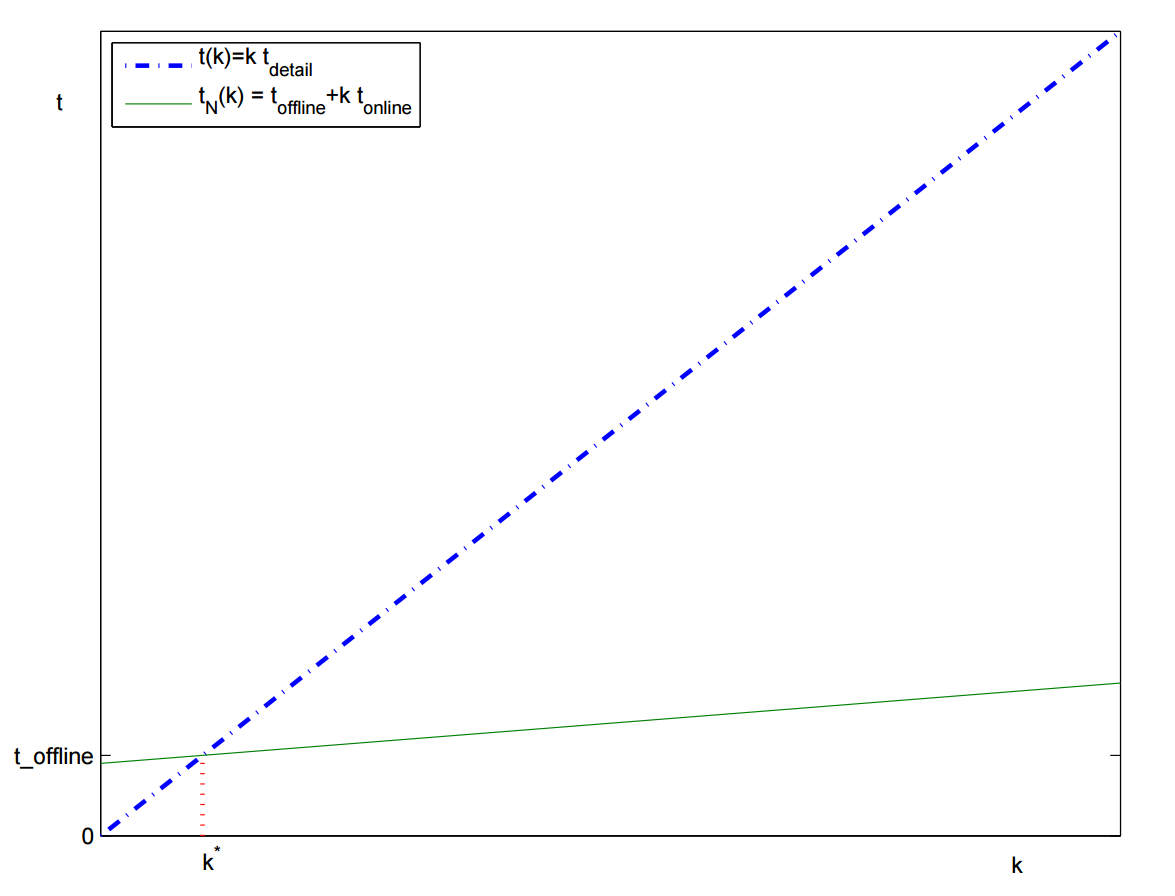
\includegraphics[width = 0.5 \textwidth]{Bilder/Laufzeiten.png}
		\caption{Laufzeiten mit wachsender Anzahl an Simulationen.}{(aus B. Haasdonk, Reduzierte-Basis-Methoden, Skript zur Vorlesung SS 2011, Universität Stuttgart, IANS-Report 4/11, 2011.)}
		\label{fig:Laufzeiten}
	\end{figure}
	\end{itemize}
\end{bem}

\begin{bem}[Keine Unterscheidung zwischen $u$ und $u_h$]
	Erinnerung: Wir unterscheiden (meistens) nicht in Notation zwischen $u_h$ (FEM-Lösung) und $u$ (Sobolev-Raum Lösung). Dies kann nun begründet werden:
	\begin{enumerate}
		\item Die Online-Phase ist unabhängig von $H = \dim(X)$, daher kann $H$ beliebig groß und damit $u_h$ beliebig präzise gemacht werden durch geeignete Diskretisierung mit genügend feinem Gitter, so dass $u$ und $u_h$ praktisch ununterscheidbar sind ($||u - u_h ||$ beliebig klein aber $(P_N(\mu))$ schnell lösbar).
		\item In der Praxis wird Reduktionsfehler den Gesamtfehler dominieren, der (FEM-)Diskretisierungsfehler spielt untergeordnete Rolle.
		\[
			\epsilon := ||u - u_h|| \ll ||u_h - u_N||
		\]
		\[
			\Rightarrow ||u_h - u_N|| - \epsilon \leq \underbrace{||u-u_N||}_{\text{theoretisch das Ideal}} \leq \overbrace{||u_h - u_N||}^{\text{berechenbar}} + \epsilon
		\]
		also kontrollieren wir durch Fehlerschranken für $||u_h - u_N||$ bis auf $\epsilon$ auch den eigentlich interessanten Fehler $||u - u_N||$.
	\end{enumerate}
\end{bem}

\subsection{Offline-/Online- Zerlegung für Fehlerschranken/Effektivitätsschranken}

Für schnelle Berechnung der Fehlerschranken \& Effektivitätsschranken benötigen wir Zerlegung für
\begin{itemize}
	\item Duale Norm des Residuums $|| r(\pdot ; \mu)||_{X'} = ||v_r||$ für alle Fehlerschranken
	\item Duale Norm des Ausgabefunktionals $|| l(\pdot;\mu)||_{X'}$ für $\Delta_{N,s}(\mu)$
	\item Norm $||u_N (\mu) ||_X$ der RB-Lösung für relativen Energienormfehlerschätzer $\Delta_N^{en, rel}$.
	\item Untere/obere Schranke $\alpha_{LB}(\mu)$ bzw. $\gamma_{UB} (\mu)$ für Koerzivitäts- bzw. Stetigkeitskonstante für Fehlerschätzer bzw. Effektivitätsschranken.
\end{itemize}
Separierbarkeit von $(P(\mu))$ überträgt sich auf Residuum

\begin{satz}[Separierbare Parameter-Abhängigkeit für $r(\pdot;\mu)$]
\label{3.22}
	Seien $a, f$ sep. parametrisch. Nach Riesz existieren $v_f^q \in X$ mit $\dotp{v_f^q}{ v} = f^q(v) \,\,\, \forall v \in X, \, q=1,...,Q_f$ und $v_a^{q,n} \in X$ mit $\dotp{v_a^{q,n}}{ v} = a^q (\phi_n,v), \, v \in X, \, q=1,...,Q_a, n=1,...,N$
	Setze $Q_r := N Q_a + Q_f$ und Aufzählung von $\{v_a^{q,n},v_f\}$ durch
	\[
		(v_r^1,...,v_r^{Q_r}) := (v_f^1,...,v_f^{Q_f},v_a^{1,1},...,v_a^{Q_a,1},v_a^{1,2},...,v_a^{Q_a,2},...,v_a^{Q_a,N})
	\]
	Für $\mu \in \mathcal{P}$ sei $u_N = \sum_{n=1}^N u_{Nn} \phi_n$ Lösung von $(P_N(\mu))$ und hiermit definiere
	\begin{align*}
		(\Theta_r^1(\mu),...,\Theta_r^{Q_r}(\mu)) := (\Theta_f^1(\mu),...,\Theta_f^{Q_f}(\mu),-\Theta_a^{1}(\mu),...,-\Theta_a^{Q_a}(\mu)u_{N1},-\Theta_a^{1}(\mu)u_{N2},... \\
		...,-\Theta_a^{Q_a}(\mu)u_{N2},...,-\Theta_a^{Q_a}(\mu)u_{NN})
	\end{align*}
	Mit $r^q(\pdot) := \dotp{v_r^q}{ \pdot} \in X', \, q = 1,...,Q_r$ sind $r(\pdot;\mu)$ und $v_r(\mu)$ separierbar parametrisch via
	\[
		r(\pdot;\mu) = \sum_{q=1}^{Q_r} \Theta_r^{q}(\mu) \cdot r^q(\pdot), \qquad v_r(\mu) = \sum_{q=1}^{Q_r} \Theta_r^{q}(\mu) \cdot v_r^q \qquad \forall \mu \in \mathcal{P}
	\]
\end{satz}

\begin{proof}
	Definition und Linearität ergibt:
	\begin{align*}
		\dotp{v_r(\mu)}{v} = r(v;\mu) &= f(v;\mu) - a(u_N(\mu),v;\mu) \\
		&= \sum_q \Theta_f^q(\mu) f^q (v) - \sum_q \sum_n \Theta_a^q (\mu) u_{Nn} a^q(\phi_n,v) \\
		&= \underbrace{\dotp{\sum_q \Theta_f^q (\mu) v_f^q - \sum_q \sum_n \Theta_a^q (\mu) u_{Nn} v_a^q}{ v}}_{\sum \Theta_r^q (\mu) v_r^q} \\
		&= \sum_{q=1}^{Q_r} \Theta_r^q (\mu) r^q(v) \qquad \forall v \in X
		\label{eq:3.5}
	\end{align*}
\end{proof}

Offensichtlich Berechnung von Riesz-Repräsentant notwendig, dies geschieht durch Ausnutzen der Endlichdim. von $X = \op{span}\{\psi_i\}_{i=1}^Ĥ$ und $K := (\dotp{\psi_i}{\psi_j})_{i,j=1}^H$

\begin{satz}[Berechnung von Riesz-Repr.]
	Für $g \in X'$ erhält man Koeffizientenvektor $\underbar v = (v_i)_{i=1}^H \in \R^H$ seines Riesz-Repräsentanten $v_g = \sum_{i=1}^H v_i \, \psi_i \in X$ durch lösen von
	\begin{align}
		K \underbar v = \underline{g}
	\end{align}
	mit Vektor $\underline{g} := (g(\psi_i))_{i=1}^H \in \R^H$
\end{satz}

\begin{proof}
	Für jedes $u = \sum_{i=1}^H u_i \, \psi_i \in X$ mit Koeffizientenvektor $\underbar u = (u_i)_{i=1}^H$ erhalten wir
	\[
		g(u) = g(\sum u_i \, \psi_i) = \sum u_i \, g(\psi_i) = \underbar u^T \underline{g} \overset{\ref{eq:3.5}}{=} \underbar u^T K \underbar v = \dotp{u}{v_g}
	\] 
\end{proof}

\begin{bem}
	\ref{eq:3.5} ist typischerweise dünn besetzt, also mit iterativen LGS-Lösern berechenbar.
\end{bem}

\begin{kor}[Offline-/Online- für Residuen-Norm]
\label{3.24}
	(Offline:) Nach Offline von $(P_N(\mu))$ gemäß \ref{3.21} def. $G_r := (r^q (v_r^{q'}))_{q,q' =1}^{Q_r} \in \R^{Q_r \times Q_r}$ mittels Residuen-Komponenten $r^q$ und Riesz-Repr. $v_r^q$ aus \ref{3.22}
	(Online:) Für $\mu \in \mathcal{P}$ und RB-Lösung $\underbar u_N \in \R^N$ berechne Residuen-Koeff-Vektor $\underline{\Theta}_r(\mu) = (\Theta_r^1(\mu),...,\Theta_r^{Q_r} (\mu))^T \, \in \R^{Q_r}$.
	Dann gilt: 
	\begin{align}
	||v_r(\mu)||_X = ||r(\pdot;\mu)||_X = \sqrt{\underline{\Theta}_r(\mu)^T \cdot G_r \underline{\Theta}_r(\mu)}
	\label{eq:3.6}
	\end{align}
\end{kor}

\begin{proof}
	Zunächst sehen wir $G_r = (\dotp{v_r^q}{v_r^{q'}})_{q, q' = 1}^{Q_r}$. Isometrie der Riesz-Abbildung \& Separierbarkeit ergeben
	\[
		||r(\mu)||_X^2 = ||v_r(\mu)||_X^2 = \dotp{\sum_{q=1}^{Q_r} \Theta_r^q(\mu) \, v_r^q}{\sum_{q'=1}^{Q_r} \Theta_r^{q'}(\mu) \, v_r^{q'}} = \underline{\Theta}_r^T \cdot G_r \cdot \underline{\Theta}_r (\mu) 
	\]
\end{proof}

\begin{bem}[Stabilisierung durch Orthonormierung von $\{v_r^q\}$]
	Wie in \textsf{demos\_chapter3(3)} gesehen, existiert eine Genauigkeitsgrenze für Fehlerschätzer, diese liegt in numerischen Auslöschungseffekten in \ref{eq:3.6} begründet, denn $G_r$ ist potentiell schlecht konditioniert. Gemäß einer Idee von Behr \& Rave 2014 lässt sich die Genauigkeit steigern, indem die $\{v_r^q\}$ orthonormiert werden und \ref{eq:3.6} mit entsprechender Transformationsmatrix modifiziert werden.
\end{bem}

\begin{kor}[Offline-/Online- Zerlegung für $||l(\pdot;\mu)||_{X'}$]
	(Offline:) Berechne Riesz-Repr. $v_l^q \in X$ der Ausgabekommponenten, d.\,h.
	\[
		\dotp{v_l^q}{v} = l^q(v) \qquad \forall v \in X, \, q=1,...,Q_l
	\]
	und def. $G_l := (l^q(v_l^{q'})_{q, q' =1}^{Q_l}$
	(Online:) Zu $\mu \in \mathcal{P}$ berechne $\underline{\Theta}_l (\mu) := (\Theta_l^1(\mu),...,\Theta_l^{Q_l}(\mu))$ und $||l(\pdot;\mu)||_{X'} = \sqrt{\underline{\Theta}_l^T G_l \underline{\Theta}_l}$
\end{kor}

\begin{proof}
	analog zu \ref{3.24}
\end{proof}

\begin{kor}[Offline-/Online für $||u_N(\mu)||_X,\, ||u_N(\mu)||_{\mu}$]
	(Offline:) Nach der Offline-Phase von $(P_N(\mu))$ def.
	\[
		K_N := (\dotp{\phi_i}{\phi_j})_{i,j=1}^N \, \in \R^{N \times N}
	\]
	(Online:) Zu $\mu \in \mathcal{P}$ berechne $A_N(\mu)$ und $\underbar u_N(\mu)$ durch Online-Phase von $(P_N(\mu)$
	\[
		|| u_N(\mu)||_X = \sqrt{\underbar u_N^T \, K_N \, \underbar u_N}
	\]
	\[
		|| u_N(\mu)||_{\mu} = \sqrt{\underbar u_N^T \, (\frac{1}{2} (A_N(\mu) + A_N(\mu)^T)) \, \underbar u_N}
	\]
\end{kor}

\begin{proof}
	\begin{align*}
		||u_N||^2 = \dotp{\sum_n u_{Nn} \phi_n \, }{ \, \sum u_{Nn'} \phi_{n'}} = \sum_{n, n'} u_{Nn} u_{Nn'} \dotp{\phi_n}[{\phi_{n'}} = \underbar u_N^T \cdot K_N \cdot \underbar u_N
	\end{align*}	
	analog für Energienorm mit $A_{N,s} := \frac{1}{2} (A_N(\mu) + A_N(\mu)^T)$
\end{proof}

\begin{bem}
	$K_N$ wieder einfach aus $K$ berechenbar (Übung).
\end{bem}

Für Fehlerschranken fehlen noch untere Schranke $\alpha_{LB} (\mu) \le \alpha (\mu)$, welche schnell berechenbar sein sollen.
Falls $a(\pdot , \pdot ; \mu)$ glm. koerziv bzgl. $\mu$ und $\bar{\alpha} < 0$ bekannt, so ist $\alpha_{LB} (\mu) := \bar{\alpha}$ gültige Wahlmöglichkeit.
In gewissen Fällen kann eine größere und damit bessere Schranke angegeben werden.

\begin{satz}[``Min-$\Theta$-Verfahren'' zur Berechnung von $\alpha_{LB}(\mu)$]
	Seien $a^q(u,u) \geq 0 \,\, \forall q,u$ und $\Theta_a^q (\mu) > 0 \,\, \forall \mu$ \\
	(Offline:) Sei $\alpha(\bar{\mu})$ für ein $\bar{\mu} \in \mathcal{P}$ verfügbar \\
	(Online:) Setze für $\mu \in \mathcal{P}$
	\[
		\alpha_{LB} (\mu) := \alpha(\bar{\mu}) \cdot \min_{q} \frac{\Theta_a^q(\mu)}{\Theta_a^q(\bar{\mu})}
	\]
	Dann gilt $0 < \alpha_{LB} (\mu) \leq \alpha(\mu)$
\end{satz}

\begin{proof}
	Wegen $0 < \alpha(\bar{\mu})$ und $0 < c(\mu) := \min\limits_q \frac{\Theta_a^q(\mu)}{\Theta_a^q(\bar{\mu})}$ gilt $ 0 < \alpha(\bar{\mu}) \cdot c(\mu) := \alpha_{LB}(\mu)$
	Folgende Argumentation ähnlich zu \ref{2.6} ii) \\
	Für alle $u \in X$ gilt
	\begin{align*}
		a(u,u;\mu) &= \sum\limits_q \Theta_a^q(\mu) \, a^q(u,u) = \sum\limits_q \frac{\Theta_a^q(\mu)}{\Theta_a^q(\bar{\mu})} \cdot \Theta_a^q(\bar{\mu}) \, a^q(u,u) \\
		&\geq \sum\limits_q \underbrace{\Bigl( \min\limits_{q'} \frac{\Theta_a^{q'}(\mu)}{\Theta_a^{q'}(\bar{\mu})} \Bigr)}_{c(\mu)} \cdot \Theta_a^q(\bar{\mu}) \, a^q(u,u) \\
		&= c(\mu) \cdot \underbrace{\sum\limits_q \Theta_a^q(\bar{\mu}) \, a^q(u,u)}_{= a(u,u;\bar{\mu})} = c(\mu) \, a(u,u;\bar{\mu}) \\
		&\overset{\text{glm. koerziv bzgl} \mu}{\geq} c(\mu) \cdot \alpha(\bar{\mu}) \cdot ||u||^2 \\
		&= \alpha_{LB}(\mu) \cdot ||u||^2
	\end{align*}
	Also insbesondere
	\[
		\alpha(\mu) = \inf\limits_u \frac{a(u,u;\mu)}{||u||^2} \geq \alpha_{LB}(\mu)
	\]
\end{proof}

\begin{bem} \beginwithlistbem
	\begin{itemize}
		\item ``Min-$\Theta$'' kann für Thermischen Block angewandt werden
		\item obiges gilt auch für nichtsymm. $a(\pdot , \pdot)$
		\item $\alpha(\bar{\mu})$ kann mittels eines hochdimensionalen Eigenwertproblems bestimmt werden:
	\end{itemize}
\end{bem}

\begin{satz}[Berechnung von $\alpha(\mu)$ für $(P(\mu))$]
	Seien $A(\mu), \, K \in \R^{H \times H}$ wie in \ref{3.19}/\ref{3.20}. \\
	Setze $A_s(\mu) := \frac{1}{2} (A(\mu) + A(\mu)^T)$. Dann gilt
	\[
		\alpha(\mu) = \lambda_{\op{min}} (K^{-1} A_s(\mu))
	\]
	wobei $\lambda_{\op{min}}$ den kleinsten Eigenwert bezeichnet.
\end{satz}

\begin{proof}
	Sie $K = L L^T$ (z.\,B. Cholesky oder Matrix-Wurzel) und verwende $\underbar v = L^t \underbar u$:
	\begin{align*}
		\alpha (\mu) &= \inf\limits_{u \in X} \frac{a(u,u;\mu)}{||u||^2} = \inf\limits_{\underbar u \in \R^H} \frac{\underbar u^T A(\mu) \underbar u}{\underbar u^T K \underbar u} \\
		&= \inf\limits_{\underbar u \in \R^H} \frac{\underbar u^T A_s(\mu) \underbar u}{\underbar u^T K \underbar u} \\
		&= \inf\limits_{\underbar v \in \R^H} \frac{\underbar v^T L^{-1} A_s \overbrace{L^{-T}}^{\text{inv. transp.} -1 \cdot T} \underbar v}{\underbar v^T L^{-1} L L^T L^{-T} \underbar v} = \inf\limits_{\underbar v \in \R^H} \frac{\underbar v^T L^{-1} A_s L^{-T} \underbar v}{\underbar v^T \underbar v}
	\end{align*}
	Also ist $\alpha(\mu)$ Minimum eines Rayleigh-Quotionenten, also kleinster Eigenwert der symmetrischen \& positiv definiten Matrix $\bar{A_s} := L^{-1} A_s L^{-T}$ \\
	Die Matrizen $\bar{A_s}$ und $K^{-1} A_s$ sind ähnlich, da 
	\[
		L^T(K^{-1}A_s)L^{-T} = L^T L^{-T}L^{-1}A_sL^{-T} = L^{-1}A_sL^{-T} = \bar{A_s}
	\]
	Also haben sie identische Eigenwerte.
\end{proof}

\begin{bem} \beginwithlistbem
	\begin{itemize}
		\item Inversion von $K$ muss verhindert werden. Daher verwende EW-Löser, welcher nur Matrix-Vektor-Multiplikation verwendet. Sobald ein Produkt $y=K^{-1}A_s x$ erforderlich ist, löst man das System $Ky = A_s x$. Alternativ kann auch kleinster EW eines verallgemeinerten EWP $A_s \underbar u = \lambda K \underbar u$ berechnet werden.
		\item Für variationelle Form des verallg. EWP für $\infty$-dim $(P(\mu))$ siehe Patera \& Rozza
		\item Für Probleme, bei denen die Voraussetzungen von Min-$\Theta$ nicht erfüllt sind, kann ``Successive Constraint Method'' (SCM) eine Alternative darstellen.  $\leadsto$ §\ref{sec-4}
	\end{itemize}
\end{bem}

\begin{satz}[``Max-$\Theta$''-Verfahren für $\gamma_{UB}(\mu)$, symmetrisches $a(\pdot , \pdot)$]
	Sei $a$ symmetrisch, koerziv, separierbar parametrisch mit $a^q$ positiv semidefinit und $\Theta_a^q > 0 \, \, \forall q,u$ \\
	(Offline:) Sei $\bar{\mu} \in \mathcal{P}$ und $\gamma(\bar{\mu})$ berechnet \\
	(Online:) Setze für $\mu \ in \mathcal{P}: \gamma_{UB}(\mu) := \gamma(\bar{\mu}) \max\limits_q \frac{\Theta_a^q(\mu)}{\Theta_a^q(\bar{\mu})}$. Dann gilt 
	\[
		\gamma_{UB}(\mu) \leq \gamma_{UB} (\mu) < \infty
	\]
\end{satz}

\begin{proof}
	Übung.
\end{proof}

\begin{bem}[Komplexitäten]
	Durch die angegebenen Berechnungsverfahren ist vollständige Offline-/Online-Zerlegung der RB-Lösung, Fehlerschranken und Effektivitätsschranken erreicht (Offline unabh. von $\mu$, Online unabh. von $H$). Komplexitäten für $\Delta_N(\mu), \Delta_{N,s}(\mu)$:
	\begin{itemize}
		\item Offline: $\O(H^3 + H^2 (Q_f + Q_l + N Q_a) + H Q_l^2 + H(Q_f + NQ_a)^2$ für EWP für $\alpha(\bar{\mu})$,
			Riesz-Repräsentanten für $f^q$, $l^q$, $a^q(\phi_n,\pdot)$ und Matrix $G_l$ und $G_r$
		\item Online: $\O((Q_f+N Q_a)^2 + Q_l^2 + Q_a)$ für Berechnung von $\norm{v_r(\pdot;\mu)}$, $\norm{l(\pdot;\mu)}_{X'}$ und $\alpha_{LB}(\mu)$ durch Min-$\Theta$.
			Problematisch ist quadratische Abhängigkeit von $Q_f$, $Q_l$, $N Q_a$, welches diese Größen in der Praxis stark einschränkt.
	\end{itemize}
\end{bem}

\paragraph{demos\_chapter3(4)} Beispiel-Lauf von Reduktionsschritten in RBmatlab.

\begin{itemize}
	\item Vorteilhafte Eigenschaften einer Basis $\Phi_N$: orthogonal für numerische Stabilität, Hierarchie, so dass Basisvektoren nach Relevanz geordnet sind, d.h. $(X_{N'})_{N'=1}^{N}$, $X_{N'} = \op{span}\{\phi_1, \dots, \phi_{N'}\}$ soll Sequenz von ``optimalen'' Räumen sein, damit durch Variation von $N'$ eine Fehlerkontrolle erlaubt.
	\item Probleme (\ref{eq:3.7}), (\ref{eq:3.8}) stellen schwierige nichtlineare Optimierungsprobleme dar. Um zu praktischer Basisgenerierung zu kommen, werden verschiedene Vereinfachungen gemacht:
	\begin{itemize}
		\item ``Snapshotbasierte'' Räume: Statt $Y \subset X$ beliebig, wird $Y = \op{span}\{u(\mu^i)\}_{i=1}^N$ mit unbekanntem $\{\mu^i\}_{i=1}^N$ gesucht. 
		\item ``Diskretisierung des Parameterraumes''. Statt $\mu \in \mathcal{P}$ wird Maximum bzw. Mittelung nur über $\mu \in \mathcal{S}_{train}$ durchgeführt, wobei $\mathcal{S}_{train} = \{\mu^i\}_{i=1}^n \subset \mathcal{P}$ \emph{endliche} Menge von Trainingsparametern $\mu$ (z.\,B. Punkte eines äquidistanten Gitters oder zufällig gewählte Parameter oder mittels adaptiven Verfahren gewählt.
		\item Statt eines Fehlermaßes, welches echte Lösung $u(\mu)$ erfordert, wird häufig ein Fehlerschätzer gewählt, welcher sehr viel schneller auswertbar ist.
		\item Das resultierende vereinfachte Optimierungsproblem kann approximativ minimiert werden, indem statt simultan über $\{\mu^i\}_{i=1}^N$ zu optimieren, einzelne Basisvektoren der Reihe nach durch Optimierung bestimmt werden (``Greedy-Verfahren'')
	\end{itemize}
\end{itemize}

\begin{defn}[Kolmogorov $n$-Weite]
Sei $\mathcal{M} \subseteq X$ kompakte Teilmenge. Zu einem abgeschlossenen Unterraum $Y \subseteq X$ nennen wir
\[
	d(Y,\mathcal{M}) := \sup_{v \in \mathcal{M}} \inf_{w \in Y} ||v-w|| = \sup_{v \in \mathcal{M}} ||v-P_Yv||
\]
den \emph{Abstand} von $Y$ zu $\mathcal{M}$. Für $n \in N$ nennen wir
\[
	d_n(\mathcal{M}) := \inf_{Y \subset X , \dim(Y) = n} d(Y,\mathcal{M})
\]
die \emph{Kolmogorov $n$-Weite} der Menge $\mathcal{M}$. Als Abschwächung definieren wir
\[
	\bar{d}_n(\mathcal{M}) := \inf_{Y \subset \op{span}(\mathcal{M}), \dim(Y)=n} d(Y,\mathcal{M}) .
\]
\end{defn}

\begin{bem} \beginwithlistbem
	\begin{itemize}
		\item $d_n$, $\bar{d}_n$ fallen monoton.
		\item $d_n$, $\bar{d}_n$ sind rein approximationstheoretische Maße, deren Abfall die Approximierbarkeit von $\mathcal{M}$ mit linearen Unterräumen charakterisiert, unabhängig von der RB-Approximation
		\item Wenn wir für ein $(\mathcal{P}(\mu))$ Konvergenz oder sogar Konvergenzrate von $d_n(\mathcal{M})$ zeigen können, so erhalten wir ebenso Konvergenz mit mind derselben Rate via Céa \ref{3.9} für die RB-Approximation
		\[
			|| u(\mu) - u_N(\mu) || \leq \frac{\gamma(\mu)}{\alpha(\mu)} \underbrace{\inf_{v \in X_N} || u(\mu) - v ||}_{d(X_N,\mathcal{M})} \leq \frac{\bar{\gamma}}{\bar{\alpha}} d_n(\mathcal{M})
		\]
		\item Beziehung $d_n$ zu $\bar{d}_n$. Es gilt trivialerweise
		\[
			d_0(\mathcal{M}) = \bar{d}_0(\mathcal{M}) = d(0,\mathcal{M}) = \sup_{v \in \mathcal{M}} ||v||,
		\]
		\[
			d_n(\mathcal{M}) \leq \bar{d}_n(\mathcal{M}) \qquad \forall n \in \N,
		\]
		falls $n_0 := \dim(\op{span}(\mathcal{M})) < \infty, \,\, d_n(\mathcal{M}) = \bar{d}_n(\mathcal{M}) = 0 \,\, \forall n \geq n_0$
		\item Präzise Werte für $d_n$ sind selten bekannt. Für endliche Menge oder Einheitskugeln können aber exakte Werte der Schranken für $d_n$ angegeben werden.
		\item Beispiel: $\mathcal{M} := \{v \in X|||v|| \leq 1\}$ erfüllt $d_n(\mathcal{M}) = \bar{d}_n(\mathcal{M}) = 1$ für alle $n < \dim(X)$ und $d_n(\mathcal{M}) = \bar{d}_n(\mathcal{M}) = 0$ für $n \geq \dim(X)$.
		\item Beispiel: $\mathcal{M} := [−1, 1]^m \subset X := R^m$ erfüllt $d_n(\mathcal{M}) = \bar{d}_n(\mathcal{M}) = \sqrt{m−n}$ für alle $n \leq m$ und $d_n(\mathcal{M}) = \bar{d}_n(\mathcal{M}) = 0$ für $n \geq m$.
		\item Beispiel: ``Müsli-Schachtel'': $\mathcal{M}:=\prod_{i \in \N} [-2^i,2^i] \subseteq l_2 \Rightarrow d_n(\mathcal{M}) \leq C \cdot 2^{-n}$, exponentielle Konvergenz
	\end{itemize}
\end{bem}

\begin{defn}[Gram-Matrix]
Zu $\{u_i\}_{i=1}^n \subset X$ definieren wir die \emph{Gram-Matrix} als $K:=(\dotp{u_i}{u_j}_X)_{i,j=1}^n \in \R^{n \times n}$
\end{defn}

\begin{lemma}[Eigenschaften von $K$]
Für $K$ Gram-Matrix von $\{u_i\}_{i=1}^n$ gilt
\begin{enumerate}
	\item $K$ ist symmetrisch und positiv semidefinit.
	\item $\op{Rang}(K) = \dim (\op{span}\{u_i\}_{i=1}^n)$
	\item $\{u_i\}_{i=1}^n$ linear unabhängig $\Leftrightarrow K$ positiv definit
\end{enumerate}
\end{lemma}

\begin{proof}
	Übung
\end{proof}

\begin{bem}[Geometrische Information in $K$]
$K$ enthält sehr viel Information der $\{u_i\}_{i=1}^n$, insbesondere kann man mittels $K$ eine isometrische Einbettung in $\R^n$ erzeugt werden, d.\,h. es existiert $\{x_i\}_{i=1}^n \in \R^n$ mit 
\[
	\dotp{x_i}{x_j}_{\R^n} = \dotp{u_i}{u_j}_X
\] 
und 
\[
	||x_i - x_j ||_{\R^n} = ||u_i - u_j||_X
\]

Sie $K = UDU^T$ Eigenwertzerlegung mit $D= \op{diag}(\lambda_1,\dots,\lambda_n)$. Setze $(x_1,\dots,x_n):=D^{\frac{1}{2}}U^T$.
Dann:
\begin{align*}
	\dotp{x_i}{x_j}_{\R^n} &= [(D^{\frac{1}{2}}U^T)_{i,j}]^T[(D^{\frac{1}{2}}U^T)_{i,j}]  \\
	&= (UD^{\frac{1}{2}})_{i,j} (D^{\frac{1}{2}} U^T)_{i,j} \\
	&= (U)_{i,j} D^{\frac{1}{2}} D^{\frac{1}{2}} (U^T)_{i,j} = (UDU^T)_{ij} = (K)_{ij} =\dotp{u_i}{u_j}_X
\end{align*}

und

\begin{align*}
	||x_i-x_j||_{\R^n}^2 &= \dotp{x_i}{x_i}_{\R^n} - 2 \dotp{x_i}{x_j}_{\R^n} + \dotp{x_j}{x_j}_{\R^n} \\
	&= \dotp{u_i}{u_i}_{X} - 2 \dotp{u_i}{u_j}_{X} + \dotp{u_j}{u_j}_{X} = ||u_i-u_j||_X
\end{align*}

Damit können viele lineare Operationen auf $\{u_i\}_{i=1}^n$ durch geeignete Operation mit $K$ ausgedrückt werden. Z.\,B. Normberechnung in $\op{span}\{u_i\}_{i=1}^n$: (siehe auch Offline/Online für Normen)
\[
	v= \sum\limits_{i=1}^n v_i u_i \,\,\,\, , \,\,\,\, \underbar v= (v_i)_{i=1}^n \in \R^n \qquad \Rightarrow \qquad ||v||_X^2 = \underbar v^T K \cdot \underbar v
\]

\end{bem}

\subsection{Basisgenerierung}
\label{sec-3.4}

\subsubsection*{Approximation durch lineare Unterräume}

Motivation für Snapshot-basierte Verfahren:
\begin{itemize}
	\item Bestimmung eines möglichst guten $X_N$, welches $\LM$ global approximiert.
	\item Formulierung durch Optimierungsproblem, z.B.\ minimiere maximalen Fehler in Energienorm
		\begin{equation}
			\min_{\stackrel{Y \subset X}{\dim Y = N}} \max_{\mu \in \p} \norm{u(\mu)-u_N(\mu)}_\mu \label{eq:3.7}
		\end{equation} 
		oder Minimum des mittleren quadratischen Projektionsfehlers
		\begin{equation}
			\min_{\stackrel{Y \subset X}{\dim Y = N}} \int_\p \norm{u(\mu)-P_Y u(\mu)}^2 \,\mathrm{d}\mu  \label{eq:3.8}
		\end{equation} 
		oder beliebiges anderes Distanzmaß.
\end{itemize}

Wir haben bereits gesehen, dass in bestimmten Fällen fehlerfreie Approximation durch geeignete RB-Räume möglich ist

\begin{satz}[Optimales $X_N$ für Thermischer Block, $B_1 = 1$]
Sie $p \in \N, \, B_1=1, \, B_2 = p, \, \mu^i := (\mu_{min},\dots,\mu_{min})^T + e_i \cdot (\mu_{max} - \mu_{min}), i=1,\dots,p$. Dann ist $X_N := \op{span}(u(\mu^i))_{i=1}^p$ optimal in dem Sinne, dass
\[
	\inf_{v \in X_N} ||u(\mu) - v|| = \inf_{v \in X_N} ||u(\mu) - v||_{\mu} = 0 \qquad \forall \mu \in \mathcal{P}
\] 
\end{satz}

\begin{proof}
Übung.
\end{proof}

\begin{satz}[Optimales $X_N$ für $Q_a=1$]
	Sei $Q_a=1$ und o.B.d.A.\ $a(u,v;\mu) = \Theta_a^1(\mu) a^1(u,v)$ und $\Theta_a^1(\mu) > 0$. Seien $\set{\mu^i}_{i=1}^{Q_f}$ derart, dass $\set{f(\pdot;\mu^i)}_{i=1}^{Q_f}$ linear unabhängig. Dann erfüllt der Lagrange RB-Raum $X_N = \spn\seq{u(\mu^i)}_{i=1}^{Q_f}$, $\dim X_N = Q_f$ und
	\[
		\inf_{v \in X_N} \norm{u(\mu)-v} = \inf_{v \in X_N} \norm{u(\mu)-v}_\mu = 0 \quad \forall \mu \in \p
	\]

	\begin{proof} \beginwithlistbew
		\begin{enumerate}
			\item \checkmark
			\item $\spn\set{f^q}_{q=1}^{Q_f} = \spn\set{f(\pdot;\mu^i)}_{i=1}^q$
				\begin{itemize}
					\item[``$\supseteq$''] ist klar weil $f(\pdot;\mu^i) = \sum_{q=1}^{Q_f} \Theta_f^q f^q(\pdot)$
					\item[``$=$''] aus Dimensionsbetrachtung
						\begin{align*}
							\dim\left( \spn\set{f(\pdot;\mu^i)}_{i=1}^{Q_f} \right) &= Q_f\\
							\dim\left( \spn\set{f^q}_{q=1}^{Q_f} \right) &\leq Q_f
						\end{align*}
						$\Rightarrow$ folgt $\dim\left( \spn\set{f^q}_{q=1}^{Q_f} \right) = Q_f$ Gleichheit beider Räume
				\end{itemize}
			\item Zeige nun exakte Approximation in $X_N$.\\
				Zu $\mu \in \p$ existiert wegen ii) $c(\mu) = \seq{c_i(\mu)}_{i=1}^{Q_f}$ mit
				\[
					f(\pdot;\mu) = \sum_{i=1}^{Q_f} c_i(\mu) f(\pdot;\mu^i) \tag{$*$}
				\]
				Damit ist dann $u(\mu) := \sum c_i(\mu) \frac{\Theta_a^q(\mu^i)}{\Theta_a^q(\mu)} u(\mu^i)$ Lösung von $\prob$:
				\begin{align*}
					a(u(\mu),v;\mu) &= \Theta_a^1(\mu) a^1(\sum c_i(\mu) \frac{\Theta_a^1(\mu^i)}{\Theta_a^1(\mu)} u(\mu^i), v)\\
					&= \sum c_i(\mu) \underbrace{\Theta_a^1(\mu^i) a^1(u(\mu^i),v)}_{=a(u(\mu^i),v;\mu^i)}\\
					&= \sum c_i(\mu) f(v;\mu^i) \stackrel{(*)}{=} f(v;\mu)
				\end{align*}
		\end{enumerate}
	\end{proof}
\end{satz}

Für die folgende Aussage referenzieren wir Fink \& Rheinboldt: On the Error Behavior of the Reduced Basis Technique for Nonlinear Finite Element Approximations, ZAMM, 63:21-28, 1983.

\begin{satz}[Lokale exponentielle Konvergenz]
	Sei $\mu^0 \in U \subset \p \subset \R$ und $u(\mu)$ analytisch in Umgebung $U$. Sei $X_{k,\mu^0}$ der Taylor-RB-Raum für $k \in \N$. Dann existiert ein $B_\delta(\mu^0) \subset U$ und $C > 0$, so dass
	\[
		\inf_{v \in X_{k,\mu^0}} \norm{u(\mu)-v} \leq C |\mu-\mu^0|^{k+1} \quad \forall \mu \in B_\delta(\mu^0)
	\]

	\begin{proof}
		Taylor-Entwicklung
		\begin{align*}
			u(\mu) &= \sum_{i=0}^\infty \frac{\partial^i}{\partial\mu^i} u(\mu^0) \frac{1}{i!} (\mu-\mu^0)^i\\
			&= \underbrace{\sum_{i=0}^k \frac{\partial^i}{\partial\mu^i} u(\mu^0) \frac{1}{i!} (\mu-\mu^0)^i}_{v_k(\mu)} + \underbrace{\sum_{i=k+1}^\infty \frac{\partial^i}{\partial\mu^i} u(\mu^0) \frac{1}{i!} (\mu-\mu^0)^{i-(k+1)} (\mu-\mu^0)^{k+1}}_{w_k(\mu)}
		\end{align*}
		Sei $\delta < 1$ so dass $B_\delta(\mu^0) \subset U$ und $C' := \sup_i \norm{\frac{\partial^i}{\partial\mu^i} u(\mu^0) \frac{1}{i!}} < \infty$. Dann gilt für $\mu \in B_\delta(\mu)$
		\begin{align*}
			\norm{w_k(\mu)} &\leq \sum_{i=k+1}^\infty \norm{\frac{\partial^i}{\partial\mu^i} u(\mu^0) \frac{1}{i!}} \cdot |\mu-\mu^0|^{i-k+1} \leq C' \sum_{i=k+1}^\infty |\mu-\mu^0|^{i-(k+1)}\\
			&\leq C' \frac{1}{1-|\mu-\mu^0|} \leq C' \frac{1}{1-\delta} =: C\\
			\inf_{v \in X_{k,\mu^0}} \norm{u(\mu)-v} &\leq \norm{u(\mu)-v_k(\mu)} = \norm{w_k(\mu) \cdot (\mu-\mu^0)^{k+1}} \leq C |\mu-\mu^0|^{k+1}
		\end{align*}
	\end{proof}
\end{satz}

Die folgende Aussage basiert auf Maday \& Patera \& Turinici: Global a priori convergence theory for reduced-basis approximations of single-parameter symmetric coercive elliptic partial differential equations. C.R.\ Acad.\ Sci., Paris, Ser.\ 1, 335, 289-294, 2002.

\begin{satz}[Globale exponentielle Konvergenz, $p=1$] \label{3.36}
	Sei $\p = [\mu_{min},\mu_{max}] \subset \R^+$ mit $\mu_{max} > 1$ genügend groß und $\mu_{min} = \frac{1}{\mu_{max}}$
	\[
		a(u,v;\mu) = \mu a^1(u,v) + a^2(u,v)
	\]
	mit $a^1$, $a^2$ symmetrisch positiv semidefinit und $f \in X'$ sei nicht parametrisch. Zu $N \in \N$, $N \geq 2$ seien
	\[
		\mu_{min} = \mu^1 < \dots < \mu^N = \mu_{max}
	\]
	logarithmisch äquidistant, d.h.\
	\[
		\ln(\mu^{i+1}) - \ln(\mu^i) = \frac{\ln(\mu_{max})-\ln(\mu_{min})}{N-1} = \delta_N
	\]
	und $X_N = \spn\set{u(\mu^i)}_{i=1}^N$ zugehöriger Lagrange RB-Raum. Dann existiert $N_0$ so dass für alle $N \geq N_0$ gilt
	\begin{equation}
		\frac{\norm{u(\mu)-u_N(\mu)}_\mu}{\norm{u(\mu)}_\mu} \leq \mu_{max}^2 e^{\frac{-N-1}{N_0-1}} \quad \forall \mu \in \p
	\end{equation}
\end{satz}

\begin{bem} \beginwithlistbem
	\begin{itemize}
		\item Voraussetzungen sind z.B.\ für einen thermischen Block mit $B_1 = 2$, $B_2 = 1$ erfüllt, wenn $\mu_2 = 1$ konstant gehalten wird und nur $\mu_1 = \mu$ variiert.
		\item Verallgemeinerung für $p > 1$ existiert.
		\item Satz \ref{3.36} liefert sogar die exponentielle Konvergenz des Approximationsfehlers und damit der Weiten $d_N$, $\bar d_N$.
	\end{itemize}
\end{bem}

\begin{kor}[Exponentielle Konvergenz von $d_N$, $\bar d_N$]
	Unter den Voraussetzungen von \ref{3.36} gilt insbesondere mit $C > 0$ unabhängig von $N$
	\[
		\inf_{v\in X_N} \norm{u(\mu)-v} \leq C \cdot e^{\frac{-N-1}{N_0-1}} \quad \forall \mu \in \p, N \geq N_0
	\]
	also für Kulmogorov $N$-Weite
	\[
		d_N(\LM) \leq C \cdot e^\frac{-N-1}{N_0-1} \quad \forall N \geq N_0
	\]
	und wegen $X_N \subset \spn(\LM)$
	\[
		\bar d_N(\LM) \leq C \cdot e^\frac{-N-1}{N_0-1}
	\]

	\begin{proof}
		Wegen Normäquivalenz und Beschränktheit von $u$ gilt
		\[
			\norm{u(\mu)}_\mu \leq \sqrt{\gamma(\mu)} \norm{u(\mu)} \leq \frac{\gamma(\mu)}{\alpha(\mu)} \norm{f(\mu)} \leq C', \quad \text{mit} \quad C' := \sup_{\mu \in \p} \frac{\sqrt{\gamma(\mu)}}{\alpha(\mu)} \norm{f(\mu)}
		\]
		Also folgt
		\begin{align*}
			\inf_{v\in X_N} \norm{u(\mu)-v} &\leq \norm{u(\mu)-u_N(\mu)} \leq \frac{1}{\sqrt{\alpha(\mu)}} \norm{u(\mu)-u_N(\mu)}_\mu \cdot \frac{\norm{u(\mu)}_\mu}{\norm{u(\mu)}_\mu}\\
			&\stackrel{\ref{3.36}}{\leq} \frac{\norm{u(\mu)}_\mu}{\sqrt{\alpha(\mu)}} \cdot e^\frac{-N-1}{N_0-1} \leq \underbrace{\frac{C'}{\bar\alpha}}_{=: C} \cdot e^\frac{-N-1}{N_0-1}
		\end{align*}
	\end{proof}
\end{kor}

Ziel ist Beweis von \ref{3.36}, hierzu benötigen wir jedoch einige Notationen und Hilfsaussagen.

\begin{itemize}
	\item Es sei $\dim X = H$ endlich aber beliebig groß.
		Man kann zeigen, dass die Konstante $N_0$ und Forderung an $\mu_{max}$ unabhängig von $H$ ist.
	\item Logarithmische Abbildung des Parametergebiets.
		Es sei
		\[
			\tau(z) = \ln(z)
		\]
		und damit $\hat\mu := \tau(\mu)$, $\hat\mu_{min} = \tau(\mu_{min})$, $\hat\mu_{max} = \tau(\mu_{max}) = -\hat\mu_{min}$, $\hat\p := \tau(\p)$, $\hat u(\hat\mu) := u(\tau^{-1}(\hat\mu))$, also $\hat u(\hat\mu)$ Lösung von
		\begin{equation}
			e^{\hat\mu} a^1(\hat u(\hat\mu), v) + a^2(\hat u(\hat\mu), v) = f(v) \quad \forall v \in X \label{eq:3.10}
		\end{equation}
		und dann $u(\mu) = \hat u(\tau(\mu))$.
	\item Es sei $\dotp{u}{v}_X := a(u,v;\mu=1) = a^1(u,v) + a^2(u,v)$, dann ist \eqref{eq:3.10} äquivalent zu
		\begin{equation}
			\dotp{\hat u(\hat\mu)}{v}_X + (e^{\hat\mu}-1) a^1(\hat u(\hat\mu),v) = f(v) \quad \forall v \in X \label{eq:3.11}
		\end{equation}
	\item Seien $\seq{\Upsilon_i, \lambda_i}_{i=1}^H \in (X, \R^+)$ Eigenfunktionen/-werte von verallgemeinertem EWP
		\begin{equation}
			a^1(\Upsilon_i,v) = \lambda_i \dotp{\Upsilon_i}{v}_X \quad \forall v \in X \label{eq:3.12}
		\end{equation}
		mit $0 \leq \lambda_1 \leq \dots \leq \lambda_H$, $\norm{\Upsilon_i} = 1$ ist dann $\set{\Upsilon_i}_{i=1}^H$ ONB von $X$.
		Aus \eqref{eq:3.12} mit $v = \Upsilon_i$ und positiver Semidefinitheit von $a^2$ folgt
		\[
			1 = \dotp{\Upsilon_i}{\Upsilon_i}_X = a^1(\Upsilon_i,\Upsilon_i) + a^2(\Upsilon_i,\Upsilon_i) = \lambda_i + a^2(\Upsilon_i,\Upsilon_i)
		\]
		\[
			\Rightarrow \lambda_i \in [0,1] =: \Lambda \text{ weil } \lambda_i = 1-a^2(\Upsilon_i,\Upsilon_i) \leq 1
		\]
	\item Aus Orthogonalität und \eqref{eq:3.12} folgt
		\begin{equation}
			a(\Upsilon_j,\Upsilon_i;\mu) = \underbrace{\dotp{\Upsilon_j}{\Upsilon_i}}_{\delta_{ij}} + (e^{\hat\mu}-1) \underbrace{a^1(\Upsilon_j,\Upsilon_i)}_{\lambda_i \delta_{ij}} = (1-\lambda_j+\lambda_j e^{\hat\mu}) \delta_{ij} \label{eq:3.13}
		\end{equation}
\end{itemize}

\begin{lemma}[Lösungsdarstellung]
\label{3.38}
	Die Lösung von \eqref{eq:3.10}, \eqref{eq:3.11} ist explizit gegeben durch
	\begin{equation}
		\hat u(\hat\mu) = \sum_{j=1}^H f_j \Upsilon_j g(\hat\mu,\lambda_j) \label{eq:3.14}
	\end{equation}
	mit $f_j = f(\Upsilon_j)$ und $g: \hat\p \times \Lambda \to \R^+$ definiert durch
	\begin{equation}
		g(z,\sigma) = \frac{1}{1-\sigma+\sigma e^z} \label{eq:3.15}
	\end{equation}

	\begin{proof}
		Einsetzen von \eqref{eq:3.14} in \eqref{eq:3.11} liefert für Testfunktionen $v := \Upsilon_i$
		\begin{align*}
			&\dotp{\sum_j f_j \Upsilon_j g(\hat\mu,\lambda_j)}{\Upsilon_i}_X + (e^{\hat\mu}-1) a^1\left( \sum_j f_j \Upsilon_j g(\hat\mu,\lambda_j), \Upsilon_i \right)\\
			&= \sum_j f_j g(\hat\mu,\lambda_j) \left( \dotp{\Upsilon_j}{\Upsilon_i}_X + (e^{\hat\mu}-1) a^1(\Upsilon_j,\Upsilon_i) \right)\\
			&\stackrel{\eqref{eq:3.13}}{=} \sum_j f_j g(\hat\mu,\lambda_j)(1-\lambda_j+\lambda_j e^{\hat\mu}) \delta_{ij}\\
			&= f_i g(\hat\mu,\lambda_i)\underbrace{(1-\lambda_i+\lambda_i e^{\hat\mu})}_{=\frac{1}{g(\hat\mu,\lambda_i)}} = f_i = f(\Upsilon_i) 
		\end{align*}
		also ist $\hat u(\hat\mu)$ Lösung von \eqref{eq:3.10} / \eqref{eq:3.11}.
	\end{proof}
\end{lemma}

\begin{bem}
	Im obigen Beweis wird also ausgenutzt, dass die Systemmatrix bezüglich $\set{\Upsilon_i}_{i=1}^H$ diagonal ist.
\end{bem}

\begin{lemma}[Energienorm-Darstellung in ONB]
\label{3.39}
	Mit $\mu = \tau^{-1}(\hat\mu)$ gilt für eine Funktion $w = \sum_{i=1}^H w_i \Upsilon_i$
	\[
		\norm{w}_\mu^2 = \sum_{i=1}^H \frac{w_i^2}{g(\hat\mu,\lambda_i)}
	\]

	\begin{proof}
		\[
			\norm{w}_{\mu} = a(w,w;\mu) = \sum_{i,j} w_i w_j \underbrace{a(\Upsilon_i,\Upsilon_j;\mu)}_{\mathclap{\stackrel{\eqref{eq:3.13}}{=} (1-\lambda_j+\lambda_j e^{\hat\mu}) \delta_{ij}}} = \sum \frac{w_i^2}{g(\hat\mu,\lambda_i)}
		\]
	\end{proof}
\end{lemma}

Wir benötigen (grobe) Schranken für $g$ und seinen Ableitungen bezüglich $z$.

\begin{lemma}[Schranken für $g$, $\frac{\partial^i}{\partial z^i} g$]
\label{3.40}
	Für alle $z \in \hat\p$, $\sigma \in \Lambda = [0,1]$ gilt
	\begin{enumerate}
		\item
			\[
				g(z,\sigma) \in \left[ \frac{1}{\mu_{max}}, \mu_{max} \right]
			\]
		\item
			\[
				\frac{1}{g(z,\sigma)} \in \left[ \frac{1}{\mu_{max}}, \mu_{max} \right]
			\]
		\item
			\[
				\left| \frac{\partial^i}{\partial z^i} g(z,\sigma) \right| \leq \bar C \cdot C \cdot j! \quad \text{mit} \quad \bar C = \mu_{max}, C = 2\mu_{max}^2
			\]
	\end{enumerate}

	\begin{proof}
		i) \& ii)
		\[
			\frac{1}{g(z,\sigma)} = 1 + \sigma (e^z-1) \stackrel{j=1}{\leq} e^{\hat\mu_{max}} = \mu_{max} \quad \Rightarrow \quad g(z,\sigma) \geq \frac{1}{\mu_{max}}
		\]
		Für festes $z$ minimiere $\frac{1}{g(z,\sigma) = 1+\sigma(e^z-1)}$ bezüglich $\sigma$
		\[
			\min_{\sigma \in [0,1]} \frac{1}{g(z,\sigma)} = \begin{cases}
				1 & z = 0 \quad (\sigma \text{ beliebig})\\
				1 & z > 0 \quad (\sigma = 0)\\
				e^z & z < 0 \quad (\sigma = 1)
			\end{cases}
		\]
		\[
			\frac{1}{g(z,\sigma)} \geq \min_{\sigma,z} \frac{1}{g(z,\sigma)} = e^{\hat\mu_{min}} = \mu_{min} = \frac{1}{\mu_{max}} \quad \Rightarrow \quad g(z,\sigma) \leq \mu_{max}
		\]
		iii) Wir zeigen per Induktion, dass $\frac{\partial^i}{\partial z^i} g(z,\sigma)$ sich darstellen lässt als
		\begin{equation}
			\frac{\partial^i}{\partial z^i} g(z,\sigma) = \sum_{k=2}^{j+1} \beta_k^j \sigma^{(k-1)} e^{(k-1)z} g^k(z,\sigma), \quad j \geq 1 \label{eq:3.16}
		\end{equation}
		mit
		\begin{equation}
			\left.
			\begin{array}{l}
				\beta_2^1 := -1\\
				\beta_2^{j+1} = \beta_2^j = -1\\
				\beta_k^{j+1} = \beta_k^j (k-1) - \beta_{k-1}^j(k-1), \quad k = 3,\dots,j+1\\
				\beta_{j+2}^{j+1} := -(j+1) \beta_{j+1}^j
			\end{array}
			\right\} \label{eq:3.17}
		\end{equation}
		Denn für $j = 1$ erhält man
		\[
			\frac{\partial}{\partial z} g(z,\sigma) = \frac{-\sigma e^z}{(1-\sigma-\sigma e^z)^2} = -e^z \sigma g^2(z,\sigma)
		\]
		also mit \eqref{eq:3.16} $\beta_2^1 = -1$.
		\paragraph*{Induktionsschritt}
		\begin{align*}
			\frac{\partial^i}{\partial z^i} g(z,\sigma) &= \frac{\partial}{\partial z} \left( \sum_{k=2}^{j+1} \beta_k^j \sigma^{(k-1)} e^{(k-1)z} g^k(z,\sigma) \right)\\
			&= \sum_{k=2}^{j+1} \beta_k^j \sigma^{(k-1)} \bigg( e^{(k-1)z} \frac{\partial}{\partial z} \underbrace{g^k(z,\sigma)}_{\mathclap{= kg^{k-1}(z,\sigma) \cdot \underbrace{\frac{\partial}{\partial z} g(z,\sigma)}_{=-\sigma e^z g^2(z,\sigma)}}}+(k-1)e^{(k-1)z} g^k(z,\sigma) \bigg)\\
			&= \sum_{k=2}^{j+1} \beta_k^j \sigma^{(k-1)} \left[ -\sigma e^{kz} k \cdot g^{k+1}(z,\sigma) + (k-1) e^{(k-1)z} g^k(z,\sigma) \right]\\
			&= \sum_{k=2}^{j+1} \beta_k^j (k-1) \sigma^{(k-1)} e^{(k-1)z} g^k(z,\sigma) + \sum_{k=3}^{j+2} \beta_{k-1}^j \sigma^{(k-1)} \cdot \left( -\sigma e^{(k-1)z} (k-1) g^k(z,\sigma) \right)\\
			&= \underbrace{\beta_2^j \sigma e^z g^2(z,\sigma)}_{k = 2} + \sum_{k=3}^{j+1} \left( \beta_k^j(k-1) - \beta_{k-1}^j(k-1) \right) \sigma^{(k-1)} e^{(k-1)z} g^k(z,\sigma)\\
			&\quad \underbrace{- \beta_{j+1}^j (j+1) \sigma^{j+1} e^{(j+1)z} g^{j+2}(z,\sigma)}_{``k=j+2``}
		\end{align*}
	Für $j \geq 1$ setze $S_j := \sum\limits_{k=2}^{j+1} |\beta_k^j|$ und zeige per Induktion, dass
	\[
		S_j \leq 2^j \cdot j! \qquad j \geq 1
	\]
	Für j = 1 ist $S_j =1 \leq 2^1 \cdot 1! = 2$ also Induktionsanfang.
	Gelte Behauptung für $j \geq 1$. Dann gilt:
	\begin{align*}
		|\beta_2^{j+1}| &= 1 \\
		|\beta_k^{j+1}| &< (j+1)(|\beta_k^j| + |\beta_{k-1}^j|) \qquad k=3,\dots,j+1 \\
		|\beta_{j+2}^{j+1}| &= (j+1) |\beta_{j+1}^j| \\
		\Rightarrow S_{j+1} = \sum\limits_{k=2}^{j+2} |\beta_k^{j+1}| &\leq 2 (j+1) S_j \overset{i.A.}{\leq} 2 (j+1) 2^j \cdot j! = 2^{j+1} (j+1)!
	\end{align*}
	Damit folgt (iii):
	\begin{align*}
	|\frac{\partial^i}{\partial z^i} g(z,\sigma)| &= |\sum\limits_{k=2}^{j+1} \beta_k^j \sigma^{(k-1)} e^{(k-1)z} g^k(z,\sigma)| \\
	&\leq \underbrace{(\sum\limits_{k=2}^{j+1} |\beta_k^j|)}_{\leq 2^j \cdot j!} \underbrace{\sup_k |\sigma^{(k-1)} e^{(k-1)z} g^k(z,\sigma)|}_{\leq 1 \cdot e^{j_{\mu_{max}}^1} \cdot \mu_{max}^{j+1} = \mu_{max} (\mu_{max}^2)^j} \\
	&\leq (2 \mu_{max}^2)^j \cdot j! \cdot \mu_{max}
	\end{align*}
	\end{proof}
\end{lemma}

\begin{bem}
$g(\hat{\mu}, \lambda_i)$ sind gemäß \ref{3.38} Koeffizienten für $\hat{u}(\hat{\mu})$ in ONB Entwicklung. Entsprechend sind $\frac{\partial^j}{\partial z^j} g(z,\sigma)$ für $z=\hat{\mu}, \, \sigma = \lambda_i$ die Koeffizienten der Sensitivitätsableitung $\frac{\partial^j}{\partial \hat{\mu}^j} \hat{u}(\hat{\mu})$ in der ONB Entwicklung, also impliziert Lemma \ref{3.40} eine Beschränktheit der Sensitivitätsableitungen.
\end{bem}

\begin{lemma}[Darstellung von Fkt. aus $X_N$]
\label{3.41}
Für Koeffizientenfunktionen $\tilde{C_n}: \hat{\mathcal{P}} \rightarrow \R, \, n=1,\dots,N$
\[
	\hat{w}_N(\hat{\mu}):= \sum\limits_{n=1}^N \tilde{C_n} (\hat{\mu})\hat{u}(\hat{\mu}^n)
\]
%?? ln hier???
mit $\hat{\mu}^n := \ln\, \mu^n$ ist also $\hat{w}_N(\hat{\mu}) \in X_N$. Dann lässt sich $\hat{w}_N$ darstellen als
\[
	\hat{w}_N(\hat{\mu}) = \sum\limits_{i=1}^H f_i \Upsilon_i \tilde{g}_N(\hat{\mu},\lambda_i)
\]
wobei $\tilde{g}_N(\hat{\mu}, \sigma) := \sum\limits_{n=1}^N \tilde{C}_n(\hat{\mu}) g(\hat{\mu}^n,\sigma)$
\begin{proof}
	Aus Lösungsdarstellung \ref{3.38} folgt
	\[
		u(\mu^n) = \hat{u}(\hat{\mu}^n) = \sum\limits_{i=1}^H f_i \Upsilon_i  g(\hat{\mu}^n,\lambda_i) \qquad ,n=1,\dots,N
	\]
	Also ist
	\[
		\hat{w}_N(\hat{\mu}) = \sum_n \tilde{C}_n(\hat{\mu})\sum\limits_{i=1}^H f_i \Upsilon_i  g(\hat{\mu}^n,\lambda_i) = \sum\limits_{i=1}^H f_i \Upsilon_i  \underbrace{\sum\limits_{n=1}^N \tilde{C}_n(\hat{\mu}) g(\hat{\mu}^n,\sigma)}_{= \tilde{g}_N(\hat{\mu},\sigma)}
	\]
\end{proof}
\end{lemma}

Wir benötigen noch Lagrange-Interpolation in M aufeinanderfolgenden Punkten $\{\hat{\mu}^i,\dots,\hat{\mu}^{i+M-1}\}$: Sie $h \in C^M(\hat{\mathcal{P}})$ zu interpolierende Funktion. Es bezeichne $I_M^i : C^0 (\hat{\mathcal{P}}) \rightarrow P_{M-1}(\hat{\mathcal{P}})$ Polynominterpolation zu $\{\hat{\mu^{i+m-1}}_{m=1}^M\}$ für $M \geq 2$ und $i \in \{1,\dots,N\}$ s.\,d. $i+M \leq N+1$.

Sei $L_M^{i;m} \in P_{M-1}(\hat{\mathcal{P}})$ Lagrange-Polynom zu den Stützstellen, d.\,h.
\[
	L_M^{i;m}(\hat{\mu}^{i+m'-1}) = \delta_{m m'} \qquad \text{für} \,\,\, 1 \leq m, m' \leq M
\]
Dann ist der Interpolant darstellbar als
\[
	(I_M^i h)(\hat{\mu}) = \sum\limits_{m=1}^M L_M^{i;m}(\hat{\mu})h(\hat{\mu}^{i+m-1})
\]
Für den Interpolationsfehler gilt in $\hat{\mu} \in [\hat{\mu}^i, \mu^{i+M-1}]$
\begin{align}
	|h(\hat{\mu} - (I_M^i h)(\hat{\mu})| &\leq \underbrace{\frac{\prod\limits_{m=1}^M |\hat{\mu}-\hat{\mu}^{i+m-1}|}{M!}}_{\leq \frac{(\hat{\mu}^{i+M-1} - \hat{\mu}^i)^M}{M!} = \frac{[(M-1)\delta_N]^M}{M!}} \sup_{\hat{\mu}'} |h^{(M)}(\hat{\mu}')| \leq \frac{[(M-1)\delta_N]^M}{M!}  \sup_{\hat{\mu}'} |h^{(M)}(\hat{\mu}')|
	\label{eq:3.18}
\end{align}

(endlich:)
\begin{proof} Satz \ref{3.36}
\\ Idee: zeige Existenz eines $\hat{w}_N(\hat{\mu}) \in X_N$ s.\,d. (mit $\mu := \tau^{-1}(\hat{\mu})$)
\begin{align}
\label{eq:3.19}
	\frac{|| \hat{u}(\hat{\mu}) - \hat{w}_N (\hat{\mu}) ||_{\mu}}{|| \hat{u}(\hat{\mu}) ||_{\mu}} \leq \mu_{max}^2 \cdot e^{\frac{-(N-1)}{N_0 - 1}} \qquad \forall N \geq N_0
\end{align}
Denn dann folgt Behauptung via $||\hat{u}(\hat{\mu})||_{\mu} = || u(\mu) ||_{\mu}$ und
\[
	|| u(\mu) - u_N(\mu) ||_{\mu} = \inf_{v \in X_N} || u(\mu) - v ||_{\mu} \leq || u(\mu) - \hat{w}_N(\hat{\mu}) ||_{\mu} = || \hat{u}(\hat{\mu}) - \hat{w}_N(\hat{\mu}) ||_{\mu}
\]
Für Konstruktion eines $\hat{w}_N(\hat{\mu})$ reicht es, die Koeffizienten $\tilde{C}_n(\hat{\mu})$ zu definieren (siehe \ref{3.41}): Sei $\hat{\mu} \in \mathcal{P}$ gegeben und $M \in \{2,\dots,N\}$ wähle $i$ s.\,d. $\hat{\mu} \in [\hat{\mu}^2,\hat{\mu}^{i+M-1}] =: J_M^i$, also $|J_M^i| = (M-1) d_N$

Definiere nun $\tilde{C}_n$ durch Lagrange-Polynome zu $\{\hat{\mu}^{i+m-1}\}_{m=1}^M$:
\[
\tilde{C}_n(\hat{\mu}) = \begin{cases}
				0 & \text{falls} \,\,\, n< i \,\,\, \text{oder} \,\,\, n \geq i+M\\
				L_M^{i;n-i+1} (\hat{\mu}) & \text{falls} \,\,\, i \leq n \leq i+M-1
			\end{cases}
\]
Dann ist zugehöriges $\tilde{g}_N(\hat{\mu}, \sigma)$ aus \ref{3.41} Interpolierende im Sinne von
\[
	\tilde{g}_N(\hat{\mu}, \sigma) = (I_M^i g(\pdot,\sigma))(\hat{\mu})
\]
denn
\[
	\tilde{g}_N(\hat{\mu}, \sigma) \overset{\ref{3.41}}{=} \sum\limits_{n=1}^N \tilde{C}_n (\hat{\mu}) g(\hat{\mu}^n,\sigma) = \sum\limits_{n=i}^{i+n-1} L_M^{i;n-i+1} (\hat{\mu}) g(\hat{\mu}^n,\sigma) = (I_M^i g(\pdot,\sigma))(\hat{\mu})
\]
also insbesondere $\tilde{g}_N(\hat{\mu}^n, \sigma) = g(\hat{\mu}^n, \sigma)$.

Betrachtet man die linke Seite von (\ref{eq:3.19}) für $\hat{w}_N (\hat{\mu})$: Mit \ref{3.41} \& \ref{3.38} \& \ref{3.39} folgt
\begin{align}
	\frac{||\hat{u}(\hat{\mu}) - \hat{w}_N (\hat{\mu}) ||_{\mu}^2}{|| \hat{u}(\hat{\mu}) ||_{\mu}^2} &\overset{\ref{3.39}}{=} \frac{\sum\limits_{i=1}^H \frac{f_i^2 (g(\hat{\mu},\lambda_i) - \tilde{g}_N (\hat{\mu},\lambda_i))^2}{g(\hat{\mu},\lambda_i)}}{\sum\limits_{i=1}^H \frac{f_i^2 g(\hat{\mu},\lambda_i)^2}{g(\hat{\mu},\lambda_i)}} \notag \\ 
	&= \frac{\sum\limits_{i=1}^H f_i^2 g(\hat{\mu},\lambda_i)^2 \frac{(g(\hat{\mu},\lambda_i) - \tilde{g}_N (\hat{\mu},\lambda_i))^2}{g(\hat{\mu},\lambda_i)^2} \frac{1}{g(\hat{\mu},\lambda_i)}}{\sum\limits_{i=1}^H \frac{f_i^2 g(\hat{\mu},\lambda_i)^2}{g(\hat{\mu},\lambda_i)}} \notag \\
	&\leq \sup_{z,\sigma} \frac{(g(z,\sigma - \tilde{g}_N(z,\sigma))^2}{g(z,\sigma)^2} \cdot \frac{\sum\limits_{i=1}^H f_i^2 \frac{g(\hat{\mu},\lambda_i)^2}{g(\hat{\mu},\lambda_i}}{\sum\limits_{i=1}^H f_i^2 \frac{g(\hat{\mu},\lambda_i)^2}{g(\hat{\mu},\lambda_i}} \notag \\
	&\leq \Big( \sup_{z,\sigma} \frac{1}{g(z,\sigma)^2} \Big) \Big( \sup_{z,\sigma} (g(z,\sigma - \tilde{g}_N(z,\sigma))^2 \Big) \notag \\
	&\overset{\ref{3.40} ii)}{\leq} \mu_{max}^2 \big( \sup_{z,\sigma} |g(z,\sigma - \tilde{g}_N(z,\sigma)| \big)^2
	\label{eq:3.20}
\end{align}
Für Fehler rechts erhalte mittels Interpolationsfehlerabschätzung:
\begin{align}
	|g(z,\sigma - \tilde{g}_N(z,\sigma)| &= | g(z,\sigma) - \big(I_M^i g(\pdot, \sigma) \big) (z)| \notag \\
	& \overset{(\ref{eq:3.18})}{\leq} \frac{\big((M-1)\delta_N \big) ^M}{M!} \sup_{\hat{\mu}'} \underbrace{| \frac{\partial^M}{\partial \hat{\mu}^M} g(\hat{\mu}', \sigma) |}_{\leq \bar{C}C^M M! \text{ wegen \ref{3.40} ii)}} \notag \\
	&= \frac{\big((M-1)\delta_N \big) ^M}{M!} \cdot \bar{C}C^M M! \notag \\
	&= \big( C(M-1)\delta_N \big)^M \cdot \bar{C}
	\label{eq:3.21}
\end{align}
Bisher: $M$ beliebig. Finde nun $M_{opt} \in \{2,\dots,N\}$, welches den Fehler ``klein'' macht. Suche zunächst ein reelles $\bar{M}_{opt} \in [2,N] \subset \R$. Hierzu setze
\[
	\bar{M}_{opt} := 1+ \frac{1}{C e \delta_N}
\]
Wir sehen mit Abbkürzung $\lambda := \ln \mu_{max} - \ln \mu_{min} = 2 \ln \mu_{max}$
\begin{align*}
	\frac{1}{C e \delta_N} \geq 1 \iff  1 \geq C e \frac{\ln \mu_{max} - \ln \mu_{min}}{N-1} &\iff N -1 \geq C \cdot e \cdot \lambda \\
	&\iff N \geq C e \lambda + 1
\end{align*}
Also ist mit Forderung $N_0 \geq C \cdot e \cdot \lambda + 1$ ist $\bar{M}_{opt} \geq 2$.
Weiter:
\begin{align*}
	1 + \frac{1}{C e \delta_N} &\iff \frac{1}{C e \delta_N} \iff 1 \leq (N-1)(C e \delta_N) \\
	&\iff 1 \leq (N-1) C \cdot e \frac{\lambda}{N-1} \iff 1 \leq C e \lambda \\
	&\overset{\ref{3.40}}{\iff} 1 \leq 2 \mu_{max}^2 \cdot e \cdot 2 \ln \mu_{max}
\end{align*}
Also ist für $\mu_{max}$ genügend groß $\bar{M}_{opt} \leq N$.

Insgesamt nun also $\bar{M}_{opt} \in [2,N]$.

Wegen $C(\bar{M}_{opt} - 1) \delta_N = C \frac{1}{C e \delta_N} \cdot \delta_N = \frac{1}{e}$ folgt
\[
	\Big(C (\bar{M}_{opt} - 1) \delta_N \Big)^{\bar{M}_{opt} -1} = \left( \frac{1}{e} \right)^{\frac{1}{C e \delta_N}} = e^{- \frac{1}{C e \delta_N}} = e^{- \frac{N-1}{C e \lambda}} \leq e^{- \frac{N-1}{N_0 -1}}
\]
falls $C e \lambda \leq N_0 -1$, d.\,h. $N_0 \geq C e \lambda + 1$ (identische Forderung an $N_0$ wie zuvor). Setze nun $M_{opt} := \lfloor \bar{M}_{opt} \rfloor$ größte ganze Zahl kleiner/gleich $\bar{M}_{opt}$
\[
	\Rightarrow M_{opt} \in \{2,\dots,N\}
\]
\[
	\text{wg.} M_{opt} \leq \bar{M}_{opt} \Rightarrow C (M_{opt} - 1) \delta_N \leq C (\bar{M}_{opt} - 1 ) \delta_N \big( = \frac{1}{e} < 1 \big)
\]
\[
	\text{und} M_{opt} > \bar{M}_{opt} - 1
\]
folgt
\begin{align}
	\big( C ( M_{opt} - 1) \delta_N \big)^{M_{opt}} \leq \big( C ( \bar{M}_{opt} - 1) \delta_N \big)^{\bar{M}_{opt}} \leq e^{- \frac{N - 1 }{N_0 - 1}}
	\label{eq:3.22}
\end{align}
Damit insgesamt
\begin{align*}
	\frac{||\hat{u}(\hat{\mu}) - \hat{w}_N (\hat{\mu}) ||_{\mu}}{|| \hat{u}(\hat{\mu}) ||_{\mu}} &\overset{(\ref{eq:3.20})}{\leq} \mu_{max} \sup_{z,\sigma} |g(z,\sigma - \tilde{g}_N(z,\sigma)| \\
	&\overset{(\ref{eq:3.21})}{\leq} \mu_{max} \underbrace{\bar{C}}_{= \mu_{max}} \cdot \big( C (M_{opt} - 1) \delta_N \big)^{M_{opt}} \overset{(\ref{eq:3.22})}{\leq} \mu_{max}^2 e^{- \frac{N - 1}{N_0 - 1}}
\end{align*}
also (\ref{eq:3.19}) und damit Satz \ref{3.36} gezeigt.
\end{proof}

\begin{defn}[Gram-Schmidt]
	Seien $\{u_i\}_{i=1}^n \in X$ lin. unabh. Dann ist \emph{Gram-Schmidt Basis} $\Phi_{GR} := \{\phi_1,\dots, \phi_n\}$ definiert durch
\[
	\bar{\phi}_m := u_m - \sum\limits_{i=1}^{m-1} \dotp{u_n}{\phi_i}\phi_i \qquad, \qquad \phi_m := \frac{\bar{\phi}_m}{||\bar{\phi}_m||} \qquad, \qquad m=1,\dots,n	
\]
und $X_{GR}$ der zugehörige \emph{Gram-Schmidt RB-Raum}
\end{defn}

\begin{lemma}[Eigenschaften von $\Phi_{GR}$] \beginwithlist
\begin{enumerate}
	\item $\Phi_{GR}$ ist ONB
	\item $\op{span}\{u_i\}_{i=1}^n = X_{GR}$
\end{enumerate}
\begin{proof}
	\begin{enumerate}
		\item Normiertheit klar nach Definition \\
		Orthogonalität per Induktion: \\
		Sei $\dotp{\phi_i}{\phi_j} = 0 \,\,\, \forall \,\,\, j < i$ \\
		Dann gilt für $j < i+1$:
		\begin{align*}
			\dotp{\bar{\phi}_{i+1}}{\phi_j} &= \dotp{u_{i+1}}{\phi_j} - \sum\limits_{k=1}^{(i+1) -1} \dotp{u_{i+1}}{\phi_k} \underbrace{\dotp{\phi_k}{\phi_j}}_{\delta_{kj} \text{ sowohl für} j<i \text{ als auch} j=i}	 \\
			&= \dotp{u_{i+1}}{\phi_j} - \dotp{u_{i+1}}{\phi_j}= 0
		\end{align*}
		also auch $\dotp{\phi_{i+1}}{\phi_j} = \dotp{\frac{\bar{\phi}_{i+1}}{||\phi_{i+1} ||}}{\phi_j} = 0$
		\item ``$\supseteq$'' klar nach Konstruktion \\
		``$=$'' folgt durch Dimensionsbetrachtung:
		\[
			\dim \op{span} \{\phi_i\}_{i=1}^n = n = \dim \op{span} \{\u_i\}_{i=1}^n
		\]
	\end{enumerate}
\end{proof}
\end{lemma}

\begin{bem} \beginwithlistbem
	\begin{itemize}
		\item Algorithmus liefert also ONB, garantiert Stabilität des RB-Verfahren für symmetrisches $a(\pdot,\pdot)$ gemäß \ref{3.7}
		\item Es existiert nur triviale Approximationsaussage, z.\,B. wegen ii):
		\[
			\max_{j=1,\dots,m} \inf_{v \in X_{GR}} ||u_j - v|| = 0
		\]
		Für Teilbasis $\Phi_{GR,m} := \{\phi_1,\dots,\phi_m\}\, , \, m < n$ werden $\{u_i\}_{i=1}^m$ exakt approximiert über $\{u_i\}_{i=m+1}^n$ weiß man nichts.
		\item Basis hängt von Reihenfolge der $\{u_i\}_{i=1}^n$ ab, macht also nur Sinn, wenn diese eine natürliche Reihenfolge haben.
		\item Gram Schmidt Orthonormierung folgt häufig als ``Postprocessing'' für anderweitig erzeugte Basis, z.\,B. Lagrange-, Greedy-Basis, etc.
	\end{itemize}
\end{bem}

\begin{satz}[Berechnung von $\Phi_{GR}$ über Gram-Matrix]
	Seien $\{u_i\}_{i=1}^m \subset X$ lin. unabh., $K = (\dotp{u_i}{u_j})_{i,j=1}^n$ mit Cholesky-Zerlegung $K=LL^T$, d.\,h. $L$ untere $\Delta$-Matrix mit positiver Diagonalen. Definiere $A=(a_{ij})_{i,j=1}^n := (L^T)^{-1}$. Dann ist die Gram-Schmidt ONB $\Phi_{GR}$ äquivalent berechenbar durch
	\[
		\phi_j = \sum\limits_{i=1}^j a_{ij} u_i \qquad \text{für}	\qquad 1 \leq j \leq n
	\]
\begin{proof}
	Übung.
\end{proof}
\end{satz}

\subsubsection*{Proper Orthogonal Decomposition (POD)}

\begin{defn}[Korrelationsoperator]
\label{3.45}
Sei $\{u_i\}_{i=1}^n \subset X$. Dann definieren wir den \emph{empirischen Korrelationsoperator} $R \in L(X,X)$ durch
\[
	Ru := \frac{1}{n} \sum\limits_{i=1}^n \dotp{u_i}{u} u_i \qquad \forall \,\, u \in X
\]
\end{defn}

\begin{bem} \beginwithlistbem
	\begin{itemize}
		\item Linearität von $R$ ist klar, Beschränktheit folgt wegen
		\[
			||Ru|| \leq \frac{1}{n} \sum ||u_i||^2 ||u|| \Rightarrow ||R|| = \sup_{u \neq 0} \frac{||Ru||}{||u||} \leq \frac{1}{n} \sum ||u_i||^2 < \infty
		\]
		also $R \in L(X,X)$
		\item Wir nennen ein $A \in L(X,X)$ \emph{kompakt} falls abgeschlossenes Bild der offenen Einheitskugel, d.\,h. $\overline{A(B_1(0))}$, kompakt ist
		\item Wir nennen $A \in L(X,X)$ selbstadjungiert (genauer Hilbertraum-selbstadjungiert), falls $\dotp{Au}{v} = \dotp{u}{Av} \,\,\,\, \forall \,\, u,v \in X$
	\end{itemize}
\end{bem}

\begin{satz}[Spektralsatz]
\label{3.46}
Sie $A \in L(X,X)$ kompakt \& selbstadjungiert, dann existiert endliche oder abzählbar unendliche orthonormmiertes System von Eigenvektoren $\{\phi_i\}_{i \in I}$, $I \subseteq \N$ zu Eigenwerten $\{\lambda_i\}_{i \in I} \subset \R \backslash \{0\}$ mit
\[
	Au = \sum_{i \in I} \lambda_i \dotp{u}{\phi_i} \phi_i \qquad \forall \,\, u \in X
\]
Falls $I$ unendlich, so $\lim\limits_{i \rightarrow \infty} \lambda_i = 0$.
\begin{proof}
	z.\,B. Alt: ``lineare Funktionalanalysis'' Satz 12.12
\end{proof}
\end{satz}

\begin{satz}[POD-Basis]
Zu $\{u_i\}_{i=1}^n$ mit $R$ aus \ref{3.45} existiert orthonormierte Menge $\{\phi_i\}_{i=1}^{n'}$ von $n' \leq n$ Eigenvektoren zu reellen Eigenwerten $\lambda_1 \geq \lambda_2 \geq \dots \geq \lambda_{n'} > 0$ mit
\begin{align}
	Ru = \sum\limits_{i=1}^{n'} \lambda_i \dotp{\phi_i}{u} \phi_i
	\label{eq:3.23}
\end{align}
Für $m = 1,\dots,n'$ definieren $\Phi_{POD} := \Phi_{POD,m} := \{\phi_i\}_{i=1}^m$ als \emph{POD-Basis} und $X_{POD} := X_{POD,m} := \op{span} \Phi_{POD,m}$ als POD-Raum.
\begin{proof}
	$R$ hat endlich dimensionales Bild, also $\overline{R(B_1(0))}$ abgeschlossen, beschränkt im endlich dimensionalen Raum, also kompakt. $R$ ist selbstadjungiert, denn $\dotp{Ru}{v} = \frac{1}{n} \sum\limits_{i=1}^n \dotp{u_u}{u} \dotp{u}{v} = \dotp{u}{Rv}$. Also existiert nach Spektralsatz \ref{3.46} entsprechend endliches ONS, das (\ref{eq:3.23}) erfüllt. Dies kann insbesondere nicht unendlich sein, wegen endlichem Bild.
\end{proof}
\end{satz}

\begin{bem} \beginwithlistbem
	\begin{itemize}
		\item Die Projektion $X \rightarrow X_{POD}$ wird in der statistischen Datenanalyse auch Hotelling-Transformation, Principal Component Analysis (PCA) oder Karhunen-Loève-Trans\-formation genannt.
		\item Bezeichnung POD, als ``proper'', ist Anlehnung an das französische ``valeur propre'' für Eigenwert.
		\item Wir nennen Basisvektoren von $\Phi_{POD}$ auch POD-Moden.
	\end{itemize}
\end{bem}

\paragraph*{Illustration}

\begin{itemize}
	\item $\{\phi_i\}_{i=1}^{n'}$ ist ONB für $\op{span} \{u_i\}_{i=1}^n$ aber nicht eindeutig (VZ oder vertauschen bei mehrfachen Eigenwerten)
	\item $\phi_1$ ist Richtung höchster Varianz von $\{u_i\}_{i=1}^n$ \\
	$\phi_2$ ist Richtung höchster Varianz von $\{P_{x_{POD,1}}^\perp u_i\}_{i=1}^n$
	\item Koordinaten der Daten in der POD-Basis sind unkorreliert $\rightarrow$ Übung.
	\item $\{\phi_i\}$, $\{\sqrt{\lambda_i}\}$ sind die Hauptachsen bzw. Achsenabschnitte des Ellipsoids $\{\dotp{u}{R^{-1}u}=1\}$
	\item Falls $X=\R^H$ und $\{u_i\}_{i=1}^n$ Realisierungen von $n$ unabhängigen, identisch normalverteilten Zufallsvariablen mit Verteilung $\mathcal{N}(\mu,\Sigma) := C \cdot \exp \big(-(x-\mu)^T \Sigma (x-\mu) \big)$ mit Mittelwert $\mu = 0$, so ist $R \in \R^{H \times H}$ guter Schätzer für $\Sigma$, insbesondere $R \rightarrow \Sigma$ konvergiert für $n \rightarrow \infty$ in geeignetem Sinne.
\end{itemize}

\begin{figure}[H]
  \centering\small
    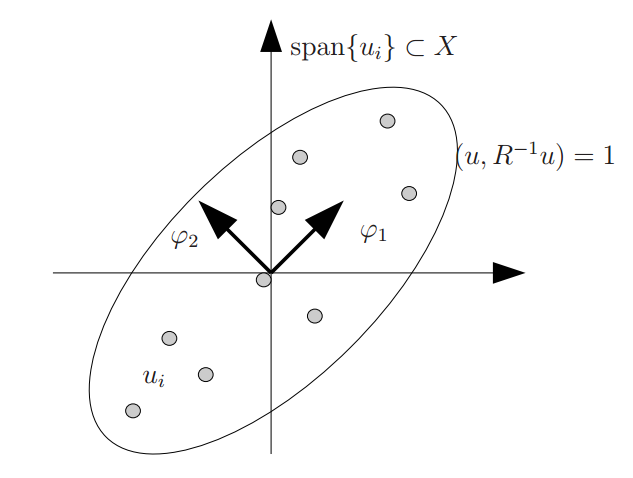
\includegraphics[width = 0.5 \textwidth]{Bilder/IllustrationPOD.png}
  \caption{Ellipsoide aus Kovarianzoperator}{(aus B. Haasdonk, Reduzierte-Basis-Methoden, Skript zur Vorlesung SS 2011, Universität Stuttgart, IANS-Report 4/11, 2011.)}
  \label{fig:IllustrationPOD}
\end{figure}

\begin{satz}[Berechnung von $\Phi_{POD}$ über Gram-Matrix]
	Sei $\{u_i\}_{i=1}^n \subset X$ und $K = \big( \dotp{u_i}{u_j}  \big)_{i,j=1}^n$. Dann sind äquivalent:
	\begin{enumerate}
		\item $\phi \in X$ ist Eigenvektor von $R$ zu Eigenwert $\lambda > 0$ mit Norm $1$ und einer Darstellung
		\[
			\phi = \sum a_i u_i \qquad \text{ mit o.\,B.\,d.\,A. } a \in \ker(K)^{\perp}
		\]
		\item $a= (a_i)_{i=1}^n \in \R^n$ ist Eigenvektor von $\frac{1}{n} K$ zu $\lambda > 0$ mit Norm $\frac{1}{\sqrt{n \lambda}}$
	\end{enumerate}
\begin{proof}
	ii) $\Rightarrow$ i)
	
	Sei $a$ Eigenvektor von $\frac{1}{n} K$ zu Eigenwert $\lambda$ mit $||a|| = \frac{1}{\sqrt{n \lambda}}$ also
	\[
		\lambda a = \frac{1}{n} K a
	\]
	Multiplikation der $i$-ten Kompoenten mit $u_i$ und Summieren ergibt
	\[
		\sum\limits_{i=1}^n u_i \lambda a_i = \sum\limits_{i=1}^n u_i \frac{1}{n} \underbrace{\big( \sum\limits_{j=1}^n \dotp{u_i}{u_j} a_j \big)}_{(K a)_i}
	\]
	Mit $\phi := \sum u_i a_i$ gilt also
	\[
		\lambda \phi = \frac{1}{n} \sum\limits_{i=1}^n u_i \dotp{u_i}{\phi} = R \phi
	\]
	Also $\phi$ Eigenvektor von $R$ zu Eigenwert $\lambda$. Für Norm folgt
	\[
		||\phi||^2 = \dotp{\sum a_i u_i}{\sum a_j u_j} = a^T \underbrace{K a}_{n \lambda a} = n \lambda \cdot ||a||^2 = 1
	\]
	K ist symmetrisch, also existiert vollständiges ONS von Eigenvektoren. $\ker(K)$ wird aufgespannt von EV zu EW 0, also $a \perp \ker(K)$, $a$ EV zu $\lambda > 0$.
	
	i) $\Rightarrow$ ii):
	
	Sie $\phi$ EV von $R$ zu EW $\lambda > 0$ und $|| \phi || = 1$. Sei $\bar{a} \in \R^n$ mit $\phi = \sum
	 \bar{a}_i u_i$ (existiert weil $\phi \in \op{Bild} (R) = \op{span} \{u_i\}_{i=1}^n$). Verschiebungen von $\bar{a}$ um $a^0 \in \ker(K)$ erhalten $\phi$:
	 \begin{align*}
	 	\phi ' := \sum (\bar{a}_i + a_i^0) u_i \Rightarrow \dotp{\phi '}{u_k} &= \dotp{\sum\limits_{i=1}^n \bar{a}_i u_i}{u_k} + \dotp{\sum_i a_i⁰0 u_i}{u_k} \\
	 	&= \dotp{\phi}{u_k} + \underbrace{\sum\limits_{i=1}^n a_i^0 \dotp{u_i}{u_k}}_{K a^0 =0} \,\,\,\, , \,\, k=1,\dots,n
	 \end{align*}
	 Also $\phi ' = \phi$.
	 
	 Wähle speziell $a := \bar{a} - P \bar{a}$, $P$ orthogonale Projektion auf $\ker(K)$.
	 \[
	 	\Rightarrow a \in \ker(K)^{\perp} \text{ , } P \bar{a} \in \ker(K) \,\,\, \Rightarrow \,\,\, \phi = \sum \bar{a}_i u_i = \sum a_i u_i
	 \]
	 i) $\Rightarrow$ ii) o.B.d.A. $a \in \ker(K^{\perp}$
	 
	 Da $\phi \in V$ zu $\lambda > 0$ gilt:
	 \[
	 	\underbrace{\frac{1}{n} \sum\limits_{i=1}^n \dotp{u_i}{\sum\limits_{j=1}^n a_i u_j}}_{R \phi} u_i = \lambda \phi = \lambda \sum_j a_j u_j
	 \]
	 Testen mit $u_k$ liefert
	 \[
	 	\frac{1}{n} \underbrace{\sum_j \dotp{u_i}{u_j} \dotp{u_i}{u_k} a_j}_{(K^2 a)_k} = \lambda \underbrace{\sum_j a_j \dotp{u_j}{u_k}}_{(Ka)_k}
	 \]
	 Also $\frac{1}{n} K^2 a= \lambda Ka$ also $Ka$ EV von $\frac{1}{n} K$ zu EW $\lambda$. Dann ist schon $a$ EV, denn $a \in \ker(K)^{\perp}$:
	 \[
	  (\ast) \,\,\, Ka (\frac{1}{n} K - \lambda) a = 0
	 \]
	 $a \in \ker(K^{\perp})$, $Ka \in \ker(K^{\perp})$ wegen Symmetrie $\dotp{Ka}{v} = \dotp{a}{Kv} = 0 \,\,\,\, \forall v \in \ker(K)$
	 
	 $\Rightarrow (\frac{1}{n} K - \lambda) a \in \ker(K)^{\perp}$
	 
	 aber auch wg. $(\ast)$ $(\frac{1}{n} K - \lambda)a \in \ker(K)$
	 
	 $\Rightarrow (\frac{1}{n} K - \lambda) a = 0$ also $a$ EV von $\frac{1}{n}K$ zu $\lambda$.
	 
	 Wie im ersten Teil gilt
	 \[
	 	1 = || \phi ||^2 = \sum a_i a_j \dotp{u_i}{u_j} = a^T K a = a^T \cdot n \lambda a = n \lambda a ||a||^2
	 \]
	 \[
		\Rightarrow ||a||= \frac{1}{\sqrt{n \cdot \lambda}}	 
	 \]
\end{proof}
\end{satz}

\begin{bem}
	Falls $X$ endlichdimensional $\dim(X) = H$, kann daher POD entweder als teures EWP f ür $R$ in $X$ (Komplexität $\mathcal{O}(H^3))$ oder, meist günstiger, als EWP für $K$ (Komplexität $\mathcal{O}(n^3))$ ermittelt werden.
	
	Bezeichnung für letzteres ist auch ``method of snapshots'' (Sirovich, 1987) oder Kernel-PCA (Schollkopf \& Smola, 2002).
	POD kann auch über Singulärwertzerlegung der Koeffizientenmatrix  berechnet werden:
\end{bem}

\begin{satz}[Berechnung für $X=\R^H$ via SVD]
	Sei $X=\R^H$ mit $\dotp{\pdot}{\pdot} = \dotp{\pdot}{\pdot}_{\R^H}$. $U = [u_1,\dots,u_n] \in \R^{H \times n}$ Snapshot-Matrix mit Rang $U = n'$ und
	\[
		U = \Phi S V^T
	\]
	eine verkürzte SVD, d.\,h. $\Phi \in \R^{H \times n'}$, $V \in \R^{n \times n'}$ orthonormale Spalten und $S= \op{diag}(\sigma_1,\dots, \sigma_{n'}) \in \R^{n' \times n'}$ ($\sigma_i$: Singulärwerte) mit $\sigma_1 \geq \sigma_2 \geq \dots \geq \sigma_{n'} \geq 0$.
	
	Dann ist $\Phi_{POD,n'} = \Phi$.
	\begin{proof}
	Sei $\Phi = (\bar{\phi_1},\dots,\bar{\phi_n})$. Nach Definition gilt $Ru = \frac{1}{n} U U^T U \,\,\, \forall u \in \R^H$. Damit ist $\bar{\phi_i}$ EV von $R$ zu $i$-ten Eigenwert $\frac{1}{n} \sigma_i^2$:
	\begin{align*}
		R \bar{\phi_i} &= \frac{1}{n} U U^T \bar{\phi_i} = \frac{1}{n} \Phi S \underbrace{V^T V}_{I} S \underbrace{\Phi^T \bar{\phi_i}}_{e_i \in \R^{n'}} \\
		&= \frac{1}{n} \Phi \underbrace{S^2 e_i}_{\sigma_i^2 e_i} = \frac{1}{n} \sigma_i^2 \bar{\phi_i}
	\end{align*}
	Die EW $\frac{1}{n} \sigma_i^2$ sind monoton fallend, also identisch sortiert wie EW von $R$, das heißt $\lambda_i = \frac{1}{n} \sigma_i^2$ und $\phi_i = \bar{\phi_i}$.
	\end{proof}
\end{satz}

\begin{bem} \beginwithlistbem
	\begin{itemize}
		\item obiges ist sehr eingänglich (``1-Zeilenbeweis''), aber algorithmisch nicht unbedingt besser, weil SVD auch durch EWP definiert (Numerik I)
		\item Verallgemeinerung für allg. HR $X$ $\rightarrow$ Übung (Blatt 5)
	\end{itemize}
\end{bem}

\begin{satz}[Approximationsfehler für $X_{POD,m}$]
Sei $\{u_i\}_{i=1}^n \subset X$ und für $Y \subset X$ Unterraum ist mittlerer quadratischer Fehler $J(Y) := \frac{1}{n} \sum\limits_{i=1}^n || u_i - P_y u_i||^2$. Dann gilt für den POD-Raum
\[
	J(X_{POD,m}) = \sum\limits_{i=m+1}^{n'} \lambda_i \qquad \text{ für } m=1,\dots,n'
\]
mit $\lambda_i$ EW von $R$.
\begin{proof}
	Sei $\Psi = \{\Psi_1,\dots,\Psi_m\}$ ONB für $Y$. Dann folgt
	\begin{align*}
		J(Y) &= \frac{1}{n} \sum\limits_{i=1}^n ||u_i - P_y u_i||^2 = \frac{1}{n} \sum\limits_{i=1}^n || u_i - \sum\limits_{j=1}^m \dotp{\Psi_j}{\u_i} \Psi_j ||^2 \\
		&= \frac{1}{n} \sum\limits_{i=1}^n ||u_i||^2 - \frac{2}{n} \sum\limits_{i=1}^n \sum\limits_{j=1}^m \dotp{u_i}{\Psi_j}^2 + \frac{1}{n} \sum\limits_{i=1}^n \sum\limits_{j,k} \dotp{\Psi_j}{u_i} \dotp{u_i}{\Psi_k} \underbrace{\dotp{\Psi_j}{\Psi_k}}_{= \sigma_jk} \\
		&= \frac{1}{n} \sum\limits_{i=1}^n ||u_i||^2 - \frac{1}{n} \sum\limits_{i=1}^n \sum\limits_{j=1}^m \dotp{u_i}{\Psi_j}^2
	\end{align*}
	Wegen $u_i \in \op{Bild} (R) = X_{POD,n'}$ ist $u_i = \sum\limits_{j=1}^{n'} \dotp{\phi_j}{u_i} \phi_j$
	\[ 
		||u_i||^2 = \sum\limits_{j,k=1}^{n'} \dotp{\phi_j}{u_i} \dotp{\phi_k}{u_i} \underbrace{\dotp{\phi_j}{\phi_k}}_{= \sigma_{jk}} = \sum\limits_{j=1}^{n'} \dotp{\phi_j}{u_i}^2
	\]
	also mittlerer quadratischer Projektionsfehler:
	\begin{align*}
		J(X_{POD,m}) &= \frac{1}{n} \sum\limits_{i=1}^n \sum\limits_{j=1}^{n'} \dotp{\phi_j}{u_i}^2 - \frac{1}{n} \sum\limits_{i=1}^n \sum\limits_{j=1}^m \dotp{u_i}{\phi_j}^2 \\
		&= \Big(  \frac{1}{n} \sum\limits_{i=1}^n \sum\limits_{j=m+1}^{n'} \dotp{\phi_j}{u_i}^2  \Big) = \frac{1}{n} \sum\limits_{i=1}^n \sum\limits_{j=m+1}^{n'} \dotp{\phi_j}{u_i} \dotp{\phi_j}{u_i} \\
		&= \sum\limits_{j=m+1}^{n'} \dotp{\phi_j}{\frac{1}{n} \sum\limits_{i=1}^n \dotp{\phi_j}{u_i} u_i} \\
		&= \sum\limits_{j=m+1}^{n'} \dotp{\phi_j}{\underbrace{R \phi_j}_{= \lambda_j \phi_j}} = \sum\limits_{j=m+1}^{n'} \lambda_j
	\end{align*}
\end{proof}
\end{satz}

\begin{satz}[Bestapproximation durch $X_{POD,m}$]
	Unter allen Räumen der Dimension $m$ ist $X_{POD,m}$ bzgl. $J$ optimal
	\[
		j(X_{POD,m}) = \inf\limits_{\substack{Y \subset X \\ \dim Y = m}} J(Y)
	\]
	\begin{proof}
		Übung.
	\end{proof}
\end{satz}

\begin{bem}[Zusammenfassung] \beginwithlistbem
	\begin{itemize}
		\item POD liefert also orthonormale Basis, garantiert Stabilität des RB-Verfahrens (bei symmetrischem $a(\pdot,\pdot)$
		\item Es existieren Approximationsaussagen bzgl. des mittleren quadratischen Projektionsfehlers, sogar Optimalität nachweisbar.
		Die POD Teilbasen ermöglichen Approximation \underline{aller} Snapshots mit Fehlerkontrolle der abgeschnittenen Eigenwerte.
		\item Die POD-Basis hängt nicht von Reihenfolge der Snapshots ab.
		\item Die POD-Basen sind hierarchisch:
		\[
			\Phi_{POD,m} \subseteq \Phi_{POD,m'} \qquad \text{ für } m \leq m'
		\]
		\item Die POD kann auch zur Erweiterung einer bestehenden ONB $\Phi$ verwendet werden, indem $\{\tilde{u}_i\}_{i=1}^n$, $\tilde{u}_i = u_i - P_{\op{span}(\Phi)} u_i$ und eine POD Basis $\tilde{\Phi}_{POD}$ hierfür berechnet wird. Dann ist $\Phi \cup \tilde{\Phi}_{POD}$ eine erweiterte/neue ONB.
		\item Man kann POD auch als inkrementelles Verfahren mit 1D-Minimierung von $J(Y)$ verstehen.
		
		Sei $\{u_i\}_{i=1}^n \subset X$. Dann definiere
		\begin{align*}
			\bar{\phi}_1 &:= POD_1 (\{u_i\}_{i=1}^n) := \op{arg inf}\limits_{\substack{\phi \in X \\ ||\phi||=1}} \frac{1}{n} \sum\limits_{i=1}^n ||u_i - \dotp{u_i}{\phi_i} \phi_i||^2 \\
			\bar{X}_1 &:= \op{span} (\bar{\phi}_1) \\
			\text{ und für } i=2,\dots,n' \\
			\bar{\phi}_i &:= POD_1(\{u_i - P_{\bar{X}_{i-1}}u_i\}), \\
			\bar{X_i} &:= \op{span} (\bar{\phi_1},\dots,\bar{\phi_i})
		\end{align*}
		Dann ist $(\bar{\phi_1},\dots,\bar{\phi_m})$ POD-Basis (aus $m$ Moden/Basisvektoren) (bis auf Rotation, Vorzeichen).
	\end{itemize}
\end{bem}

\subsubsection*{Greedy-Verfahren}

\begin{defn}[Greedy-Verfahren]
	Sei $S_{train} \subset \mathcal{P}$ ``Trainingsmenge'' von Parametern, $\Delta (Y,\mu) \in \R^+$ für Teilräume $Y \subset X$ und Parameter $\mu \in \mathcal{P}$ ein ``Fehlerindikator'' und $\epsilon_{tol} > 0$ eine Fehlertoleranz. Die Greedy-Basen $\Phi_{GRE,m}$, Greedy-Raum $X_{GRE,m}$ und Sample-Menge $S_m$ für $m=0,\dots,N$ sind iterativ definiert durch
	\[
		S_0 = \emptyset \,\, , \,\, X_{GRE,0} = \{0\} \,\, , \,\, \Phi_{GRE,0} = \emptyset \,\, , \,\, m:=0
	\]
Solange $\epsilon_m := \max\limits_{\mu \in S_{train}} \Delta(X_{GRE,m},\mu) > \epsilon_{tol}$
\begin{align*}
	\mu^{(m+1)} &:= \op{max arg}\limits_{\mu \in S_{train}} \Delta(X_{GRE,m},\mu) \\
	S_{m+1} &:= S_m \cup \{\mu^{(m+1)}\} \\
	\phi_{m+1} &:= u(\mu^{(m+1)} \text{ Lösung von } (P(\mu^{(m+1)})) \\
	\Phi_{GRE,m+1} &:= \Phi_{GRE,m} \cup \{\phi_{m+1}\} \\
	X_{GRE,m+1} &:= X_{GRE,m} + \op{span}(\phi_{m+1}) \\
	m \leftarrow m+1
\end{align*}
setze schließlich $N:=m$
\end{defn}

\begin{bem} \beginwithlistbem
	\begin{itemize}
		\item Erste  Verwendung von Greedy-Verfahren für RB: Veroy, Prud'homme, Rovas, Patera 2003, seitdem ``Standard''
		\item $\Phi_{GRE,m}$ ist Lagrange-RB zur Sample-Menge $S_m$, i. a. nicht orthonormal. Kann für numerische Stabilität mit Gram-Schmidt orthonormalisiert werden.
		\item Basen sind hierarchisch: $\Phi_{GRE,m} \subset \Phi_{GRE,m'}$, $m \leq m'$
		\item In Literatur wird Suche nach $\mu^{(1)}$ häufig umgangen, indem dieses beliebig aus $S_{train}$ gewählt wird.
		\item $S_{train}$ wird häufig als strukturierte oder zufällige Menge aus $\mathcal{P}$ mit \emph{endlich} vielen Samples gewählt.
		\item Falls $S_{train}$ zu klein, kann das RB-Modell overfitting aufweisen, d.\,h.
		\[
			\sup\limits_{\mu \in \mathcal{P}} || u(\mu) - u_N(\mu) || >> \sup\limits_{\mu \in S_{train}} || u(\mu) - u_N(\mu) ||
		\]
		\item Greedy-Verfahren ist also akkummulatives Verfahren, welches iterativ den ``schlechtest''-aufgelösten Parameter $\mu^{(m+1)}$ wählt, $u(\mu^{(m+1)}$ berechnet, und als neuen Basisvektor hinzufügt. Insofern kann dies als approximative Lösung des Optimierungsproblems
		\[
			\min\limits_{\substack{Y \subset X \\ \dim Y = N}} \max\limits_{\mu \in \mathcal{P}} \Delta (Y,\mu)
		\]
	interpretiert werden: Statt maximieren über $\mathcal{P} \leadsto	$ maximieren über $S_{train}$, statt minimieren über $X \subset X \leadsto$ iterative Sequenz von Räumen $Y = X_{GRE,m}$.
	\end{itemize}
\end{bem}

\begin{lemma}[Fehlerindikatoren, Terminieren des Verfahrens] \beginwithlist
\begin{enumerate}
	\item Falls  $|S_{train}| = n < \infty$ und für alle $\mu \in \mathcal{P}$ und $Y \subset X$ gilt
	\[
		u(\mu) \in Y \,\, \Rightarrow \,\, \Delta(Y,\mu) = 0
	\]
	so terminiert das Greedy-Verfahren mit $N \leq n$ und
	\[
		\max\limits_{\mu \in S_{train}} \Delta(X_{GRE, n} , \mu) \leq \epsilon_{tol}
	\]
	\item Dies erfüllen z.\,B.
	\[
		\Delta(Y,\mu) := ||u(\mu) - u_N(\mu)||
	\]
	\[
		\Delta(Y,\mu) := ||u(\mu) - P_y u(\mu)||
	\]
	\[
		\Delta(Y,\mu) := \Delta_N^{en} (\mu)
	\]
	oder andere Fehlerschätzer, wobei $X_N = Y$ gesetzt wird.
\end{enumerate}
\begin{proof}
	Übung.
\end{proof}
\end{lemma}

\begin{kor}[Fehleraussage]
	Für $\Delta(Y,\mu) := ||u(\mu) - u_N(\mu)||$ oder $\Delta(Y,\mu) := \Delta_{N'}$ gilt für $N' = 1,\dots,N$
	\[
		\max\limits_{\mu \in S_{train}} ||u(\mu) - u_{N'}(\mu)|| \leq \epsilon_{N'}
	\]
	\begin{proof}
		Klar nach Konstruktion.
	\end{proof}
\end{kor}

\begin{bem}[Wahl der Fehlerindikatoren] \beginwithlistbem
	\begin{itemize}
		\item Greedy-Verfahren hervorragendes Einsatzfeld für Fehlerschätzer, denn $\Delta_N(\mu)$ kann sehr schnell für alle $\mu \in S_{train}$ ausgerechnet werden, ohne dass alle $u(\mu)$, $\mu \in S_{train}$ berechnet werden müssen (im Gegensatz zu POD). Dadurch können sehr große Mengen $S_{train}$ behandelt werden. Dies erhöht die Erwartung, dass $\Phi_{GRE,N}$ auch für neue Parameter $\mu \in \mathcal{P} \backslash S_{train}$ eine gute Approximation liefert.
		\item Wahl: $\Delta(Y,\mu) := ||u(\mu) - P_y u(\mu)||$, orthogonaler Projektionsfehler
		
		Motivation: Falls dies klein, so ist mit Céa auch RB-Fehler klein
		
		Nachteile: Teuer auszuwerten, hochdimensionale Operation erfordert alle Snapshots $u(\mu)$, $\mu \in S_{train}$ müssen vorliegen, Größe von $S_{train}$ hiermit eingeschränkt.
		
		Vorteil: Terminieren ist garantiert. Approximationsraum ist entkoppelt von RB-Approximation, d.\,h. Verfahren kann angewandt werden ohne Vorliegen des RB-Verfahren und ohne Fehlerschätzer.
		\item Wahl: $\Delta(Y,\mu) := ||u(\mu) - u_N(\mu)||$, RB-Fehler
		
		Motivation: Dies ist die ultimative Größe, welche kontrolliert werden muss, z.\,B. (\ref{eq:3.7}).
		
		Nachteile: Wie bei Projektionsfehler: teuer, alle Snapshots $\mu \in S_{train}$ vorberechnen, $S_{train}$ Größe eingeschränkt.
		
		Vorteile: Terminieren ist garantiert, Verfahren kann mit RB-Verfahren angewandtwerden, für welche keine FS vorliegen.
		\item Wahl: $\Delta(Y,\mu) = \Delta_N (\mu)$ [oder Energie-/rel. Fehlerschätzer]
		
		Nachteil: Falls Fehlerschätzer den Fehler stark überschätzt, kann der RB-Raum evtl. größer als nötig sein.
		
		Vorteile: schnell auswertbar, unabhängig von $H$ denn Offline-Online. Es müssen nur $N$ Snapshots berechnet werden, $|S_{train}|$ kann sehr groß gewählt werden, Terminieren kann garantiert werden.
		\item Ziel-orientierte Indikatoren: Falls $\Delta(Y,\mu)$ als Ausgabefehler $|s(\mu) - s_N(\mu)|$ oder -Schranke $\Delta_N,s$ gewählt wird, nennt man das Verfahren ``goal-oriented''. Die Basis wird potentiell sehr klein und kann Ausgabe gut approximieren. Die Feldvariable $u$ wird jedoch nicht notwendigerweise gut approximiert.
		\item Falls $\Delta(Y,\mu)$ als Feldvariablen-Fehler $||u(\mu)-u_N(\mu)||$, PRojektionsfehler oder -schätzer gewählt wird, ist Verfahren nicht goal-oriented, die Basis wird größer sein, aber sowohl $u$ als auch $v$, als auch beliebig andere Funktionale $\tilde{s}$ gut approximiert.
	\end{itemize}
\end{bem}

\begin{bem}[Reihenfolge] \beginwithlistbem
	\begin{itemize}
		\item Greedy-Basis hängt meistens nicht von Reihenfolge der Parameter $S_{train}$ ab. Nur falls zufällig das Maximum von $\Delta(Y,\mu)$ mehrdeutig ist $\leadsto$ Praktische Lösung: Wähle ersten Parameter, der maximales $\Delta(Y,\mu)$ erzeugt.
	\end{itemize}
\end{bem}

\begin{bem}[Bestimmung der Approximationsgüte/Overfitting]
In Terminologie der Statistik/Maschinellen Lernens ist $S_{train}$ eine \emph{Trainingsmenge} und $\epsilon_N$ aus Greedy-Verfahren der sogenannten \emph{Trainingsfehler}. $S_{train}$ muss $\mathcal{P}$ gut repräsentieren, sollte möglichst groß gewählt werden. Falls $S_{train}$ zu klein, oder unrepräsentativ für $\mathcal{P}$ kann Overfitting auftreten.

Somit ist kleiner Trainingsfehler nicht hinreichend für gutes Modell. Modelle sollen daher nicht alleine anhand von Trainings-, sondern anhand unabhängiger Testmengen:
\[
	\epsilon_{test} = \max\limits_{\mu \in S_{train}} \Delta(X_N,\mu) \qquad \text{, meistens zufällige Parametermenge}
\]
\end{bem}

\begin{bem}[Monotonie] \beginwithlistbem
	\begin{itemize}
		\item Im Allgemeinen gilt nicht $\Delta(X_N,\mu) \geq \Delta(X_{n+1},\mu)$
		\item Es kann daher vorkommen, dass $(\epsilon_n)_{n=1}^N$ nichtmonoton ist.
		\item Falls Beziehung zu Bestapproximation gilt, d.\,h. für ein $C > 0$ unabhängig von $n$ gilt:
		\[
			\Delta(X_n,\mu) \leq C \cdot \inf\limits_{v \in X_n} ||u(\mu) - v||
		\]
		kann zumindest eine Beschränkung oder asymptotischer Abfall erwartet werden.
		\item In bestimmten Fällen kann Monotonie bewiesen werden:
	\end{itemize}
\end{bem}

\begin{satz}[Monotonie von $(\epsilon_n)$]
Das Greedy-Verfahren erzeugt monoton fallende Sequenzen $(\epsilon_n)_{n\geq 1}$ falls:
\begin{enumerate}
	\item $\Delta (Y,\mu) := ||u(\mu) - P_{X_n}u(\mu)||$ oder
	\item $(P)$ ist compliant, d.\,h. $l=f$ und $a$ symmetrisch und $\Delta(Y,\mu) = ||u(\mu) - u_N(\mu)||_{\mu}$
\end{enumerate}
\begin{proof}
	\begin{enumerate}
	\item klar
	\item folgt aus \ref{3.11}
	\end{enumerate}
\end{proof}
\end{satz}

\begin{bem}[Konvergenz des Greedy-Verfahrens] \beginwithlistbem
	\begin{itemize}
		\item Einige Jahre lang war Greedy-Verfahren ein in der Praxis gut funktionierendes Verfahren, jedoch ohne theoretische Erklärung wann/warum es funktioniert.
		\item Notwendiges Kriterium für Erfolg des Greedy-Verfahren: Kolmogorov $n$-Weite von $\mathcal{M}$ muss (schnell) abfallen. Sei $\Delta(Y,\mu)$ so gewählt, dass $\Delta(Y,\mu) \geq || u(\mu - P_yu(\mu)||$
		\begin{align*}
			&\Rightarrow \sup\limits_{\mu \in \mathcal{P}} \Delta(Y,\mu) \geq \inf\limits_{\substack{Y \subset X \\ \dim Y = n}} \sup\limits_{\mu \in \mathcal{P}} ||u(\mu) - P_yu(\mu)|| = d_n(\mathcal{M}) \\
		\end{align*}
		$\Rightarrow$ Falls $\Phi_{GRE,n}$ gut, muss $d_n(\mathcal{M})$ klein sein. Falls $d_n(\mathcal{M})$ nicht klein, kann $\Phi_{GRE,n}$ keine gute Approximation liefern.
		
		\item Spannend ist umgekehrte Frage, ob abfallendes $d_n$ auch hinreichend für Gelingen des Greedy-Verfahrens.
		\item Antwort auf diese Fragen wurden in letzten Jahren gegeben:
		
		(BMPPT 2012): Buffa, Maday, Patera, Prud'homme, Turinici: A-priori convergence of the greedy algorithm for the parameterized reduced basis method
		
		M2AN, 46:595-..., 2012		
		
		(BCDDPW): Binev, Cohen, Dahmen, DeVore, Petrova, Wojtaszczyk: Convergence Rates for Greedy Algorithms in Reduced Basis Methods
		
		SIAM J. Math. Anal., 43(3), 1455..., 2011.
		\item Die Hoffnung, ein Ergebnis der Form $\epsilon_n \leq c d_1(\mathcal{M})$ zu erhalten kann (ohne weitere Annahme) leider nicht erreicht werden. Dies sieht man durch Vergleich von
		\[
			\bar{d}_n(\mathcal{M}) = \inf\limits_{\substack{Y \subset \op{span}(\mathcal{M}) \\ \dim Y = n}} d(Y,\mathcal{M}) \qquad \text{und} \qquad d_n(\mathcal{M})
		\]
		Theorem 4.1 in (BCDDPW2011) besagt:
		\begin{enumerate}
			\item Für jedes $\mathcal{M}$ und $n \geq 0$ gilt $\bar{d}_n(\mathcal{M}) \leq (n+1) d_n(\mathcal{M})$
			\item Für jedes $n > 0$ und $\epsilon > 0$ existiert $\mathcal{M}$, s.\,d.
			\[
				\bar{d}_n(\mathcal{M}) \geq (n-1-\epsilon)d_n(\mathcal{M})
			\]
			\end{enumerate}
		Wegen $\epsilon_n \geq \bar{d}_n(\mathcal{M})$ und ii) ist ``direkter Vergleich'' von $\epsilon_n$ und $d_n(\mathcal{M})$ mit $C$ unabhängig von $n$ nicht möglich.
		\item Lösung ist zusätzliche Annahmen von Raten des Abfalls von $d_n$, damit können ähnliche Abfallraten für $\epsilon_n$ gezeigt werden, z.\,B. zeigen (BMPPT2012):
		
		Für $S_{train} = \mathcal{P}$ und $\Delta(Y,\mu) = ||u(\mu) - P_yu(\mu)||$:
		\[
			\epsilon_n \leq 2^{n+1}(n+1) d_n(\mathcal{M})
		\]
		Falls $d_n$ schnell genug abfällt (z.\,B. exponentiell $d_n(\mathcal{M}) \leq C \cdot e^{-\alpha n})$ so folgt dann auch exponentieller Abfall von $\epsilon_n$ (mit anderem $\alpha$)
		\item Ein verbessertes Ergebnis (ohne Faktor $(n+1)$) und ein Ergebnis für Fall algebraischer (polynomiell in $N^{-1}$) Konvergenz liefert (BCDPW), welches wir in unserer Notation formulieren (ohne Beweis).
	\end{itemize}
\end{bem}